\documentclass[aspectratio=169,11pt]{beamer}
\usetheme{Madrid}
\usepackage{amsmath, amssymb}
\usepackage{graphicx}
\usepackage{tikz}
\usepackage{comment}
\usepackage{hyperref}
\usepackage{subcaption}

\title[]{A toy model of deep learning}
\author[Corlouer]{Guillaume Corlouer}
\institute{Stormglass}
\date{}

\begin{document}
\maketitle
\begin{frame}[plain]
\centering
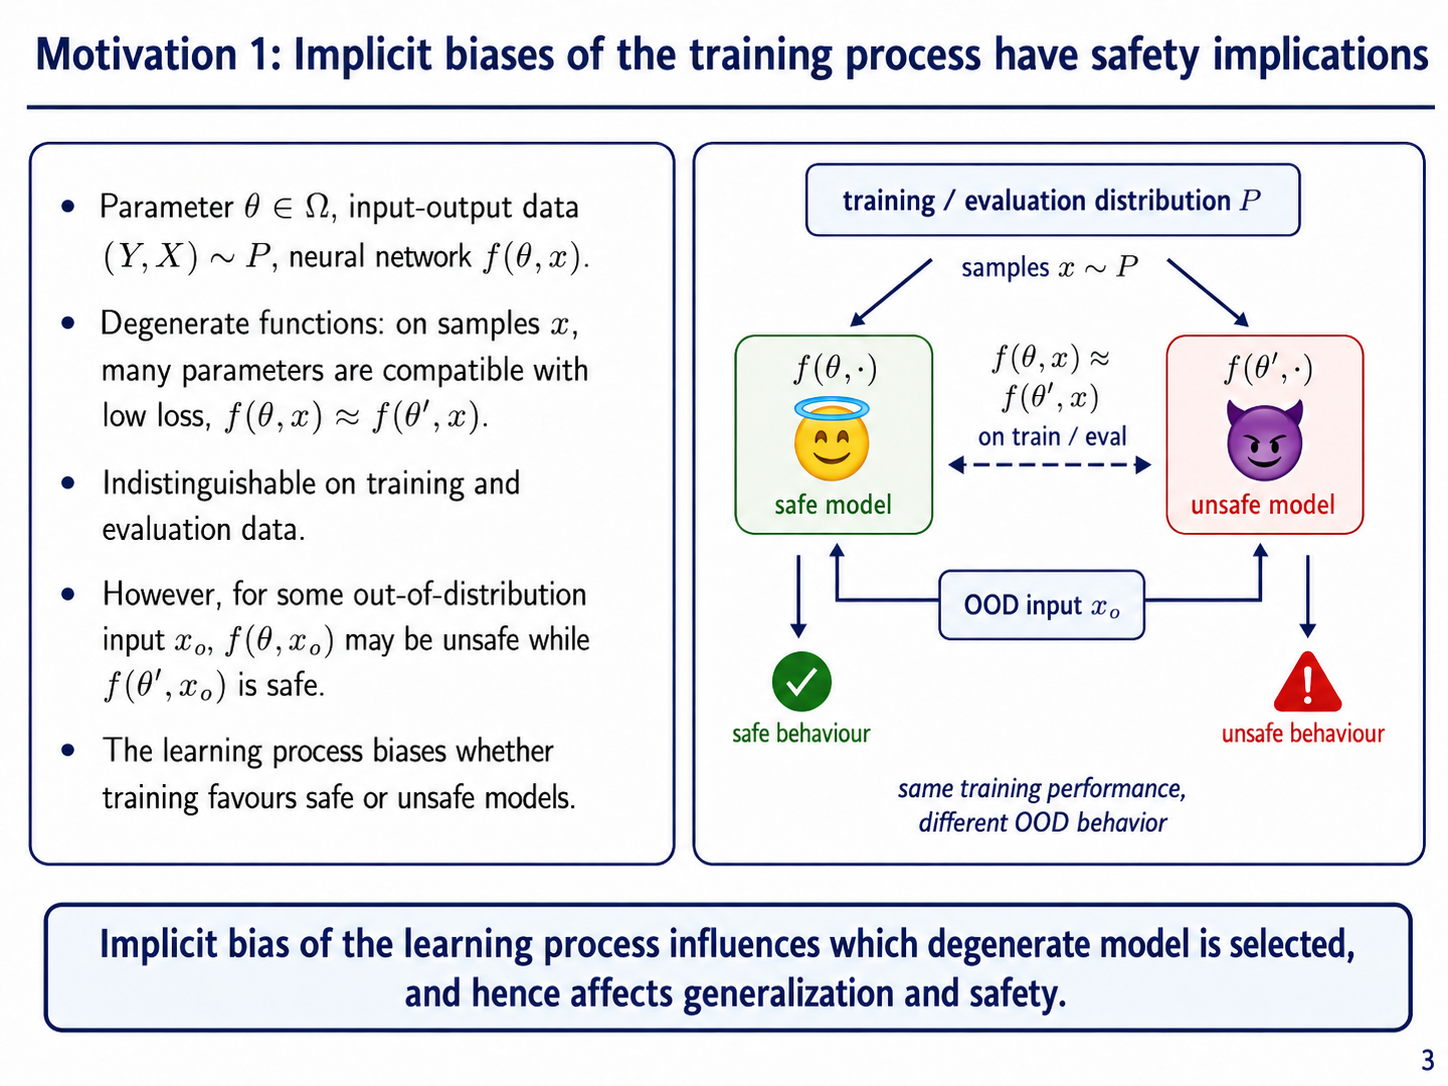
\includegraphics[width=\textwidth,height=\textheight,keepaspectratio]{figures/implicit_biases_motivation.png}
\end{frame}
\begin{frame}{Motivation 2: Interpretability over training}
\begin{itemize}
    \item Would like to know more principled observables to track
    \item Learning dynamics can help define useful observables
    \item Challenging to reverse engineer a neural network after training
    \item Structure often emerges sequentially across different timescales
    \item It may be easier to decompose a model's internal structure during training
\end{itemize}

\end{frame}
\section{Setup}
\begin{frame}[plain]
\begin{tikzpicture}[remember picture,overlay]
\node[inner sep=0pt] at (current page.center) {%
\begin{beamercolorbox}[wd=.75\paperwidth,sep=1.4em,center,rounded=true,shadow=true]{title}
{\usebeamerfont{title}\Huge Setup}
\end{beamercolorbox}
};
\end{tikzpicture}
\end{frame}
\begin{frame}[plain]
\centering
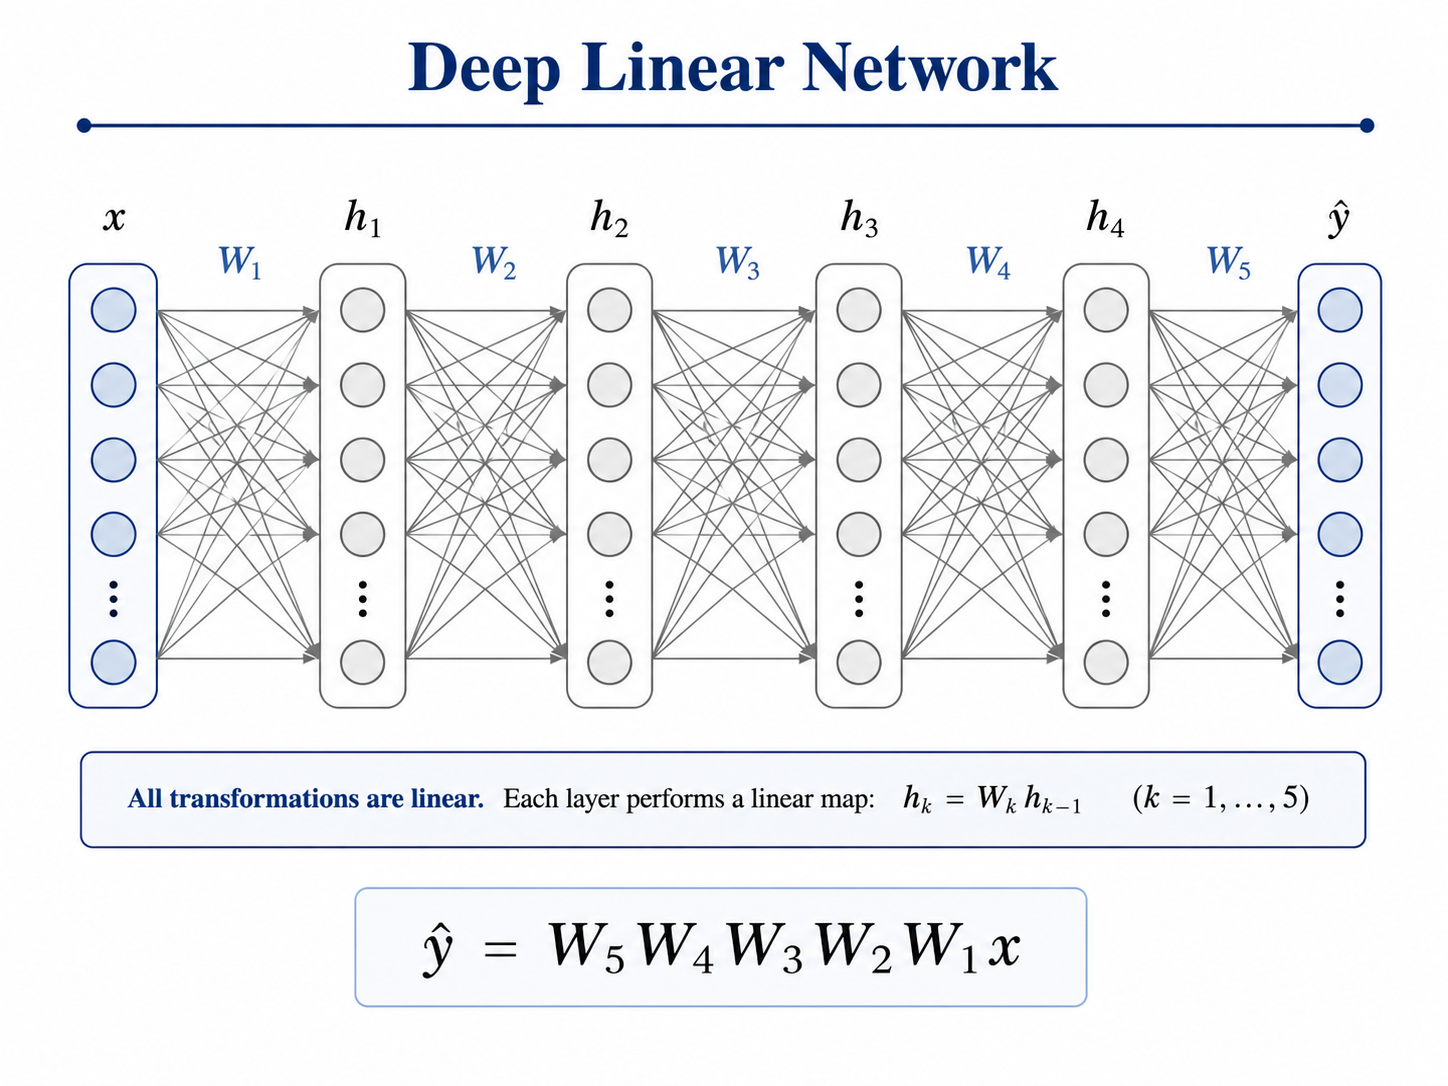
\includegraphics[width=\paperwidth,height=\paperheight,keepaspectratio]{figures/DLN_diagram.png}
\end{frame}
\begin{frame}{The harmonic oscillator of deep learning}
\begin{block}{Definition}
A $L$-layer Deep Linear Network is a function:
\begin{align*}
    f: \ & \mathbb{R}^{d_0}\times \prod_{\ell=1}^{L}\operatorname{Mat}_{d_\ell\times d_{\ell-1}}  \to \mathbb{R}^{d_L} \\
       & (x,\theta :=(W_1,\ldots,W_L)) \mapsto W_L\cdots W_1 x = Wx
\end{align*}
$d_0$ is the input dimension; $d_\ell$, $1\leq \ell \leq L$, is the width of layer $\ell$.
\end{block}
\end{frame}
\begin{frame}[plain]
\centering
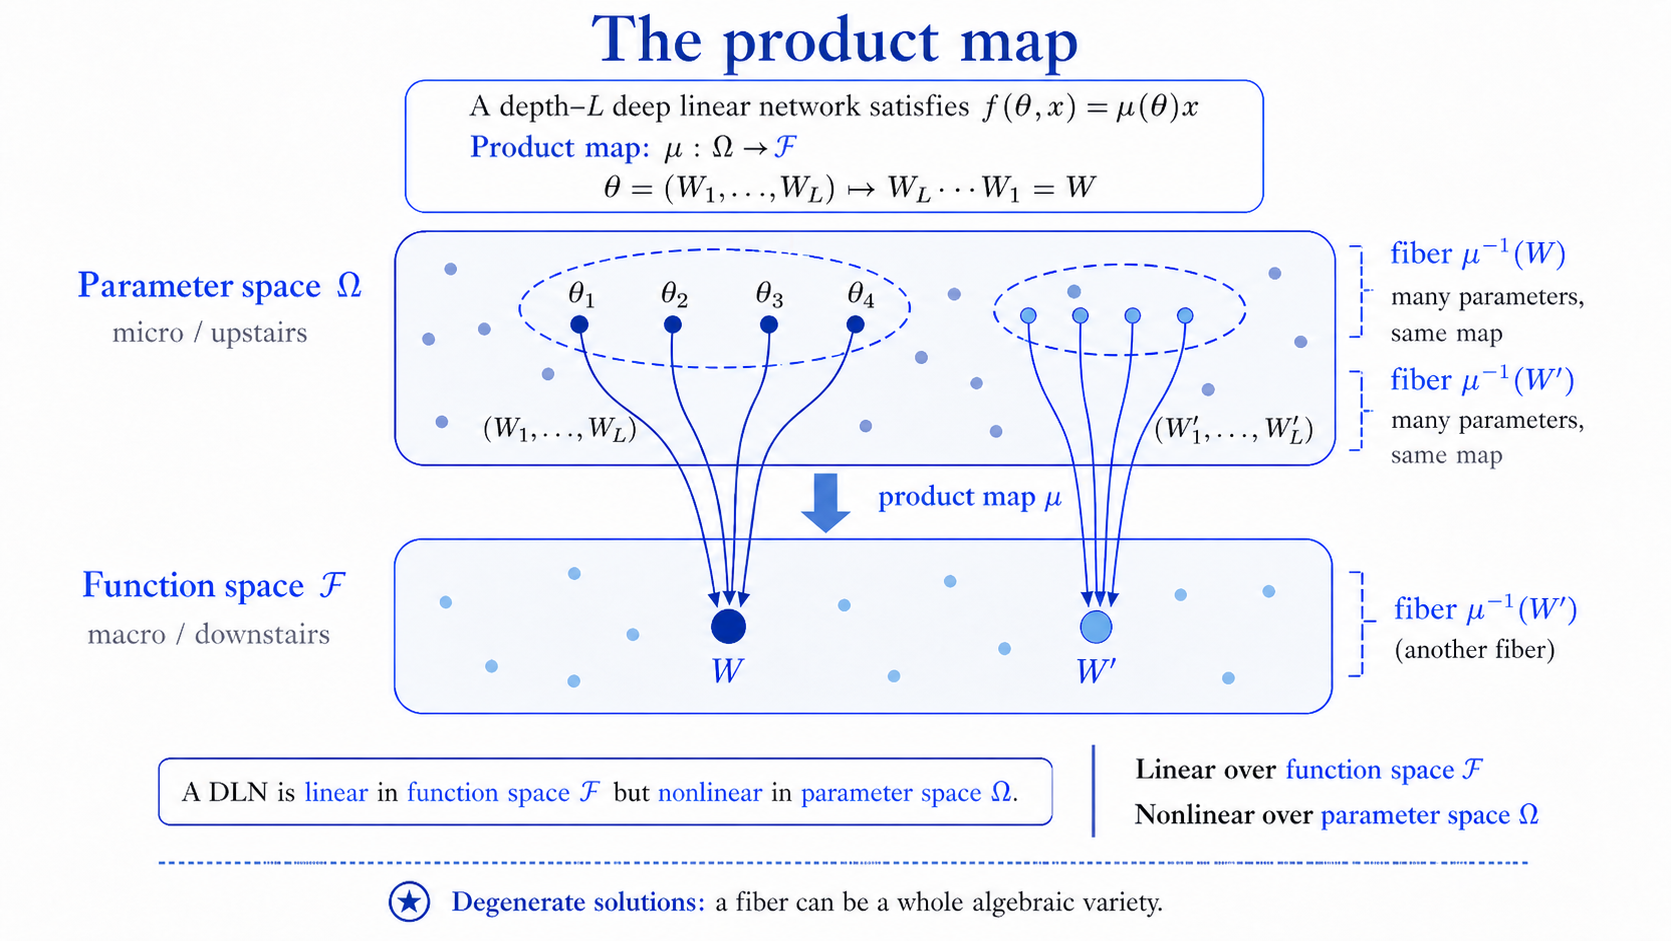
\includegraphics[width=\textwidth,height=\textheight,keepaspectratio]{figures/DLN_fiber_mult_map.png}
\end{frame}
\begin{comment}
% ---------- Slide: Product map----------
\begin{frame}{The product map}
\begin{block}{Definition}
A DLN $f(\theta,x)$ of depth $L$ satisfies $f(\theta,x)= \mu(\theta)x$ with \textit{product map} $\mu$:
    \begin{align*}
    \pi :  & \ \Omega = \operatorname{Mat}_{d_l\times d_{l-1}}\to \mathcal{F} = \operatorname{Mat}_{d_0\times d_L}\\
         \theta:=& (W_1,...,W_L) \mapsto W_L...W_1=W
\end{align*}
We note $W:=\pi(\theta)$. A DLN is linear over function space $\mathcal{F}$ and non-linear over parameter space $\Omega$.
\end{block}
Intuition: Parameter space $\Omega$ is micro (upstair) and $\mathcal{F}$ is macro (downstair). 
\\
Degenerate solutions: fiber $\mu^{-1}(\theta)$ can be a whole algebraic variety.
\end{frame}
\end{comment}
\begin{frame}{Data, loss function, training}
\begin{block}{Quadratic population loss and gradient flow}
Let $M$ be the teacher matrix, with $y=Mx$ and $x\sim \mathcal{N}(0,I)$.
The input-output covariance is $\Sigma_{YX}=M$.
\begin{equation*}
    \mathcal{L}(\theta) := \frac{1}{2} \lVert M - W_L\cdots W_1\rVert^2_F = \frac{1}{2} \lVert M - W\rVert^2_F
\end{equation*}
Initialize $\theta_0 \sim \mathcal{N}(0, \sigma^{-\gamma})$, where $\gamma$ controls the initialization scale. Then gradient flow is
\[
\dot{W}_\ell = - \nabla_{W_{\ell}} \mathcal{L}(\theta).
\]
\end{block}
Frobenius norm: $\lVert A\rVert_F:=\sqrt{\operatorname{Tr}(A^{\top}A)}$.
\\
Global minimizers achieve zero loss: $\exists \theta^{\star}\in \Omega,\ \mu(\theta^{\star}) = W^{\star} = M$.
\\
The structure of the data is encoded by $\Sigma_{YX}$.

\end{frame}
\begin{frame}
    \centering Empirical phenomena
\end{frame}
\begin{frame}{Training losses}
Initialize weights: $\theta \sim \mathcal{N}(0,\sigma^{-\frac{\gamma}{2}})$
\\
$\gamma < 1$: large initialization, linear regime (NTK)
\\
$\gamma > 1$: small initialization, saddle-to-saddle
\\
$\gamma = 1$: intermediate regime

    \begin{figure}
        \centering
        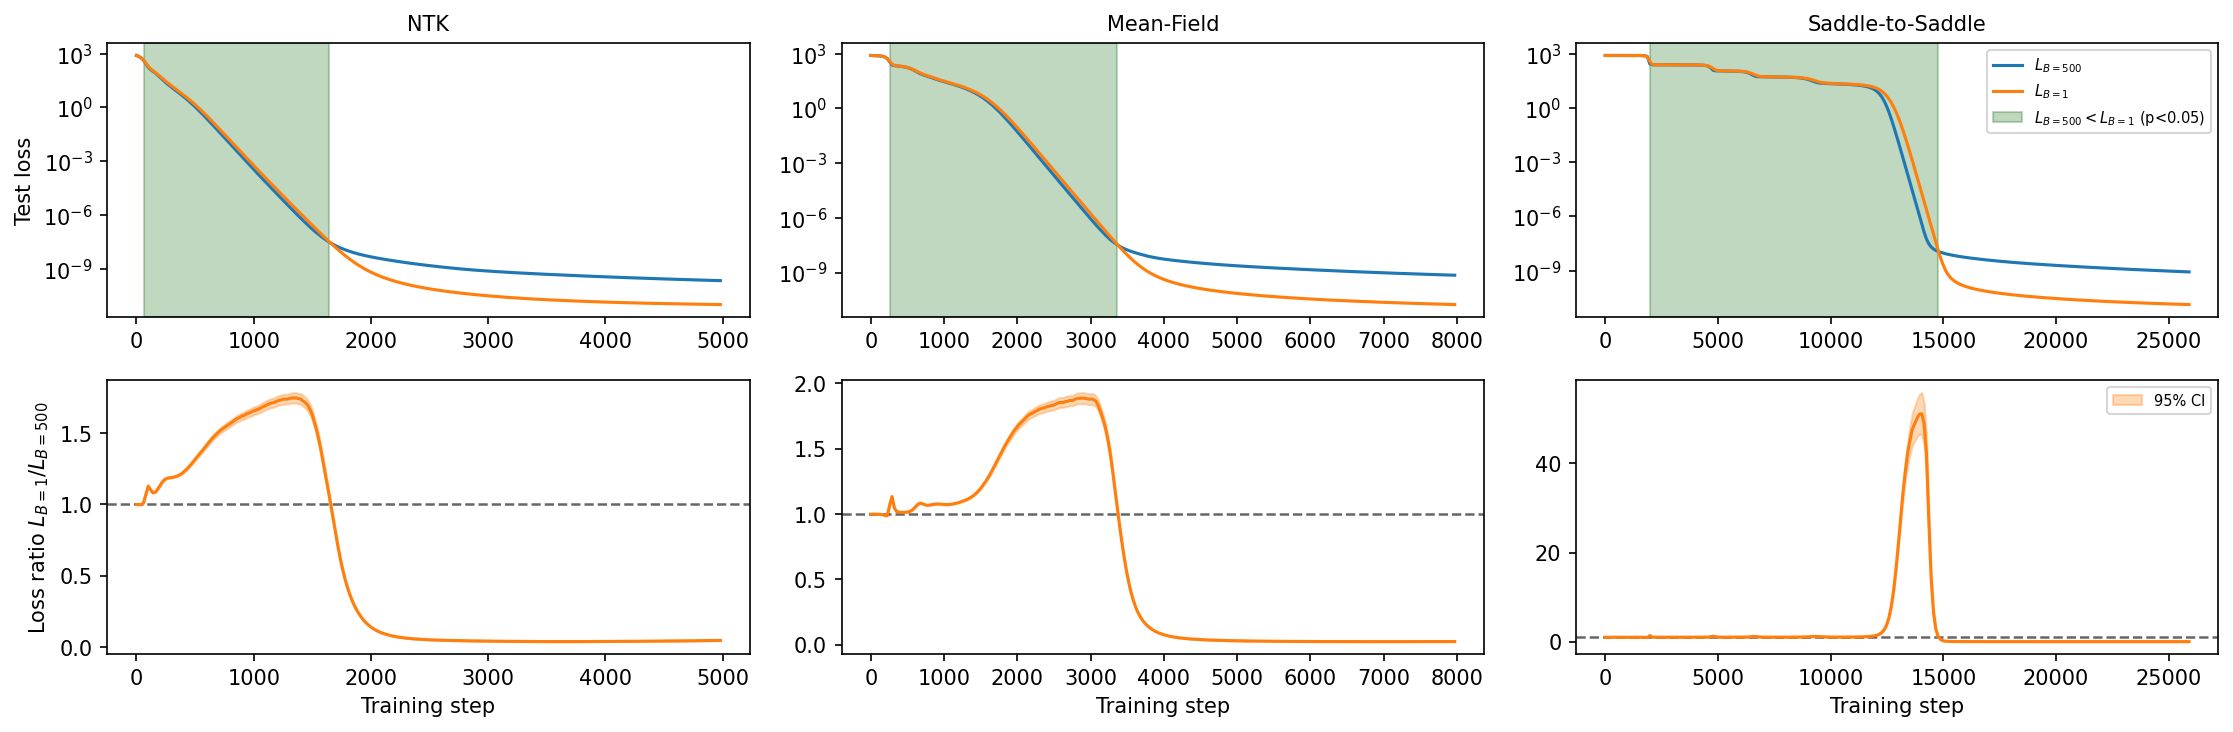
\includegraphics[width=\linewidth]{figures/DLN_losses_regimes.png}
    \end{figure}
\end{frame}

\begin{frame}{Singular values of student matrix}
    \begin{figure}
        \centering
        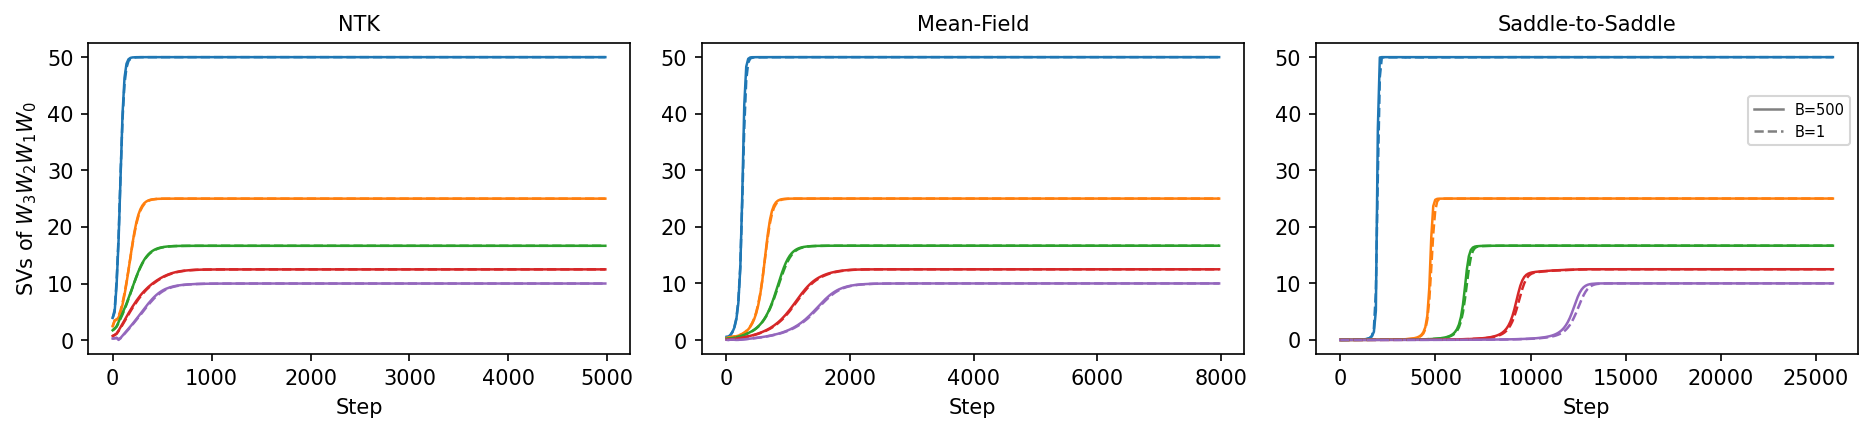
\includegraphics[width=\linewidth]{figures/DLN_sv_students.png}
    \end{figure}
\end{frame}

\begin{frame}{Singular values of individual weight matrices}
    \begin{figure}
        \centering
        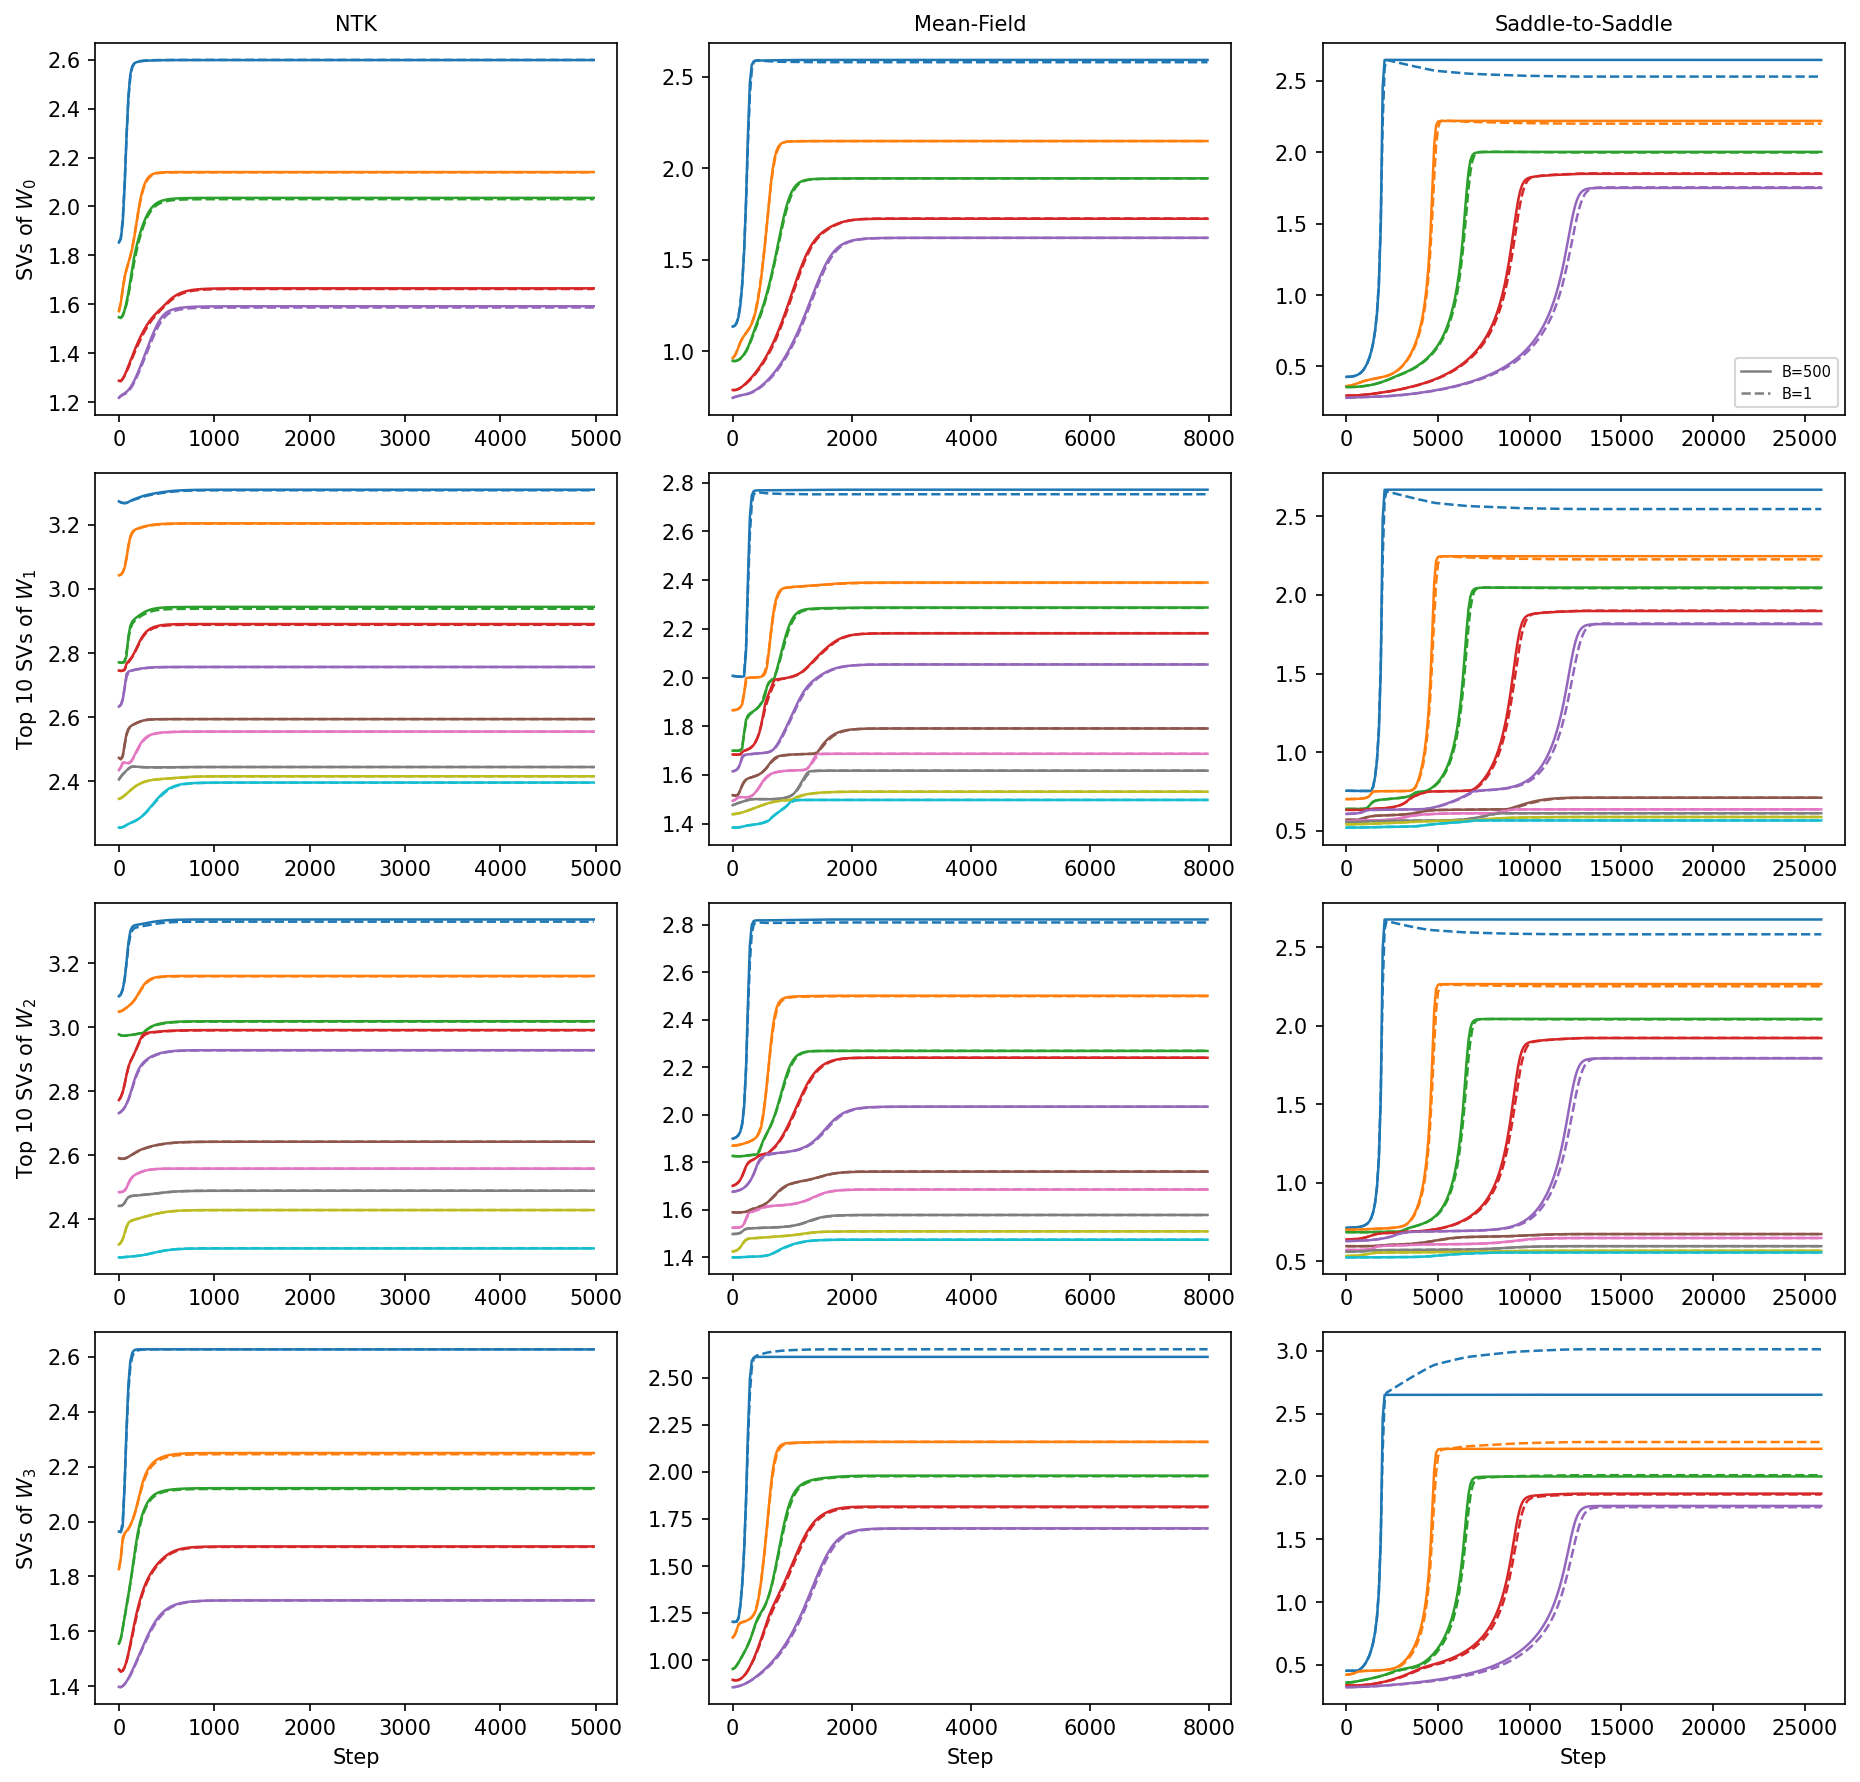
\includegraphics[width=\linewidth]{figures/DLN_individual_sv.png}
    \end{figure}
\end{frame}
\begin{frame}{Motivation}
\begin{itemize}
    \item Mathematically tractable toy model that exhibits interesting and relevant phenomena
    \item Some behaviours transfer to nonlinear architectures
    \item A first model for understanding implicit biases and weight interpretability during training
\end{itemize}
\end{frame}
\begin{frame}
    \centering Geometry
\end{frame}
% ---------- Slide: 2-layer diagonal DLN ----------
\begin{frame}{A 2-layer diagonal DLN}
\small

\begin{block}{Model and loss}
Take a 2-layer diagonal DLN of width \(2\):
\[
W_1=\operatorname{diag}(b_1,b_2),
\qquad
W_2=\operatorname{diag}(a_1,a_2),
\qquad
\theta=(W_1,W_2).
\]
Hence the student matrix is
\[
W=W_2W_1=\operatorname{diag}(a_1b_1,a_2b_2).
\]
Let the teacher be
\[
M=\operatorname{diag}(s_1,s_2),
\qquad s_1,s_2>0,
\qquad x\sim \mathcal{N}(0,I).
\]
With whitened inputs, the quadratic population loss is
\[
\mathcal L(\theta)
=
\frac12\lVert M-W\rVert_F^2
=
\frac12(a_1b_1-s_1)^2
+
\frac12(a_2b_2-s_2)^2.
\]
\end{block}
\end{frame}
\begin{frame}
\small
\begin{block}{Gradient equations}
For \(i=1,2\),
\[
\partial_{a_i}\mathcal L
=
(a_i b_i-s_i)b_i,
\qquad
\partial_{b_i}\mathcal L
=
(a_i b_i-s_i)a_i.
\]
Therefore the critical point equations are
\[
(a_i b_i-s_i)b_i=0,
\qquad
(a_i b_i-s_i)a_i=0,
\qquad i=1,2.
\]
\end{block}

\centering
\small
The two coordinates decouple: each singular direction can be analyzed independently.

\begin{block}{Coordinate-wise characterization}
For each \(i=1,2\), the critical point equations are
\[
(a_i b_i-s_i)b_i=0,
\qquad
(a_i b_i-s_i)a_i=0.
\]
Since \(s_i>0\), this implies exactly two possibilities:
\[
a_i b_i=s_i
\qquad\text{or}\qquad
a_i=b_i=0.
\]
Thus each coordinate either fits the teacher singular value or is shut off.
\end{block}

\end{frame}


% ---------- Slide: Critical points ----------
\begin{frame}{Critical points}

\begin{block}{All critical points}
\[
\begin{array}{c|c|c}
\text{Parameter conditions}
&
\text{Realized student matrix } W
&
\text{Loss}
\\
\hline
a_1b_1=s_1,\ a_2b_2=s_2
&
W=\operatorname{diag}(s_1,s_2)=M
&
\mathcal L=0
\\[0.4em]
a_1b_1=s_1,\ a_2=b_2=0
&
W=\operatorname{diag}(s_1,0)
&
\mathcal L=\frac12s_2^2
\\[0.4em]
a_1=b_1=0,\ a_2b_2=s_2
&
W=\operatorname{diag}(0,s_2)
&
\mathcal L=\frac12s_1^2
\\[0.4em]
a_1=b_1=0,\ a_2=b_2=0
&
W=0
&
\mathcal L=\frac12(s_1^2+s_2^2)
\end{array}
\]
\end{block}

\centering
\small
Critical points correspond to choosing a subset of the teacher singular values.
\\
Depth introduces three new critical points compared with the one-layer DLN loss $\mathcal{L}(W)=\lVert M - \operatorname{diag}(w_1,w_2)\rVert^2_F$.

\end{frame}

\begin{comment}
% ---------- Slide: Saddles or global minimum ----------
\begin{frame}{Global minimum and saddles}

\begin{block}{Example}
If both singular directions are fitted,
\[
a_1b_1=s_1,
\qquad
a_2b_2=s_2,
\]
then
\[
W=M=\operatorname{diag}(s_1,s_2),
\qquad
\mathcal L=0.
\]
Since \(\mathcal L(\theta)\geq 0\), these critical points are global minima.
\end{block}
\end{frame}
\end{comment}
\begin{frame}[plain]
\centering
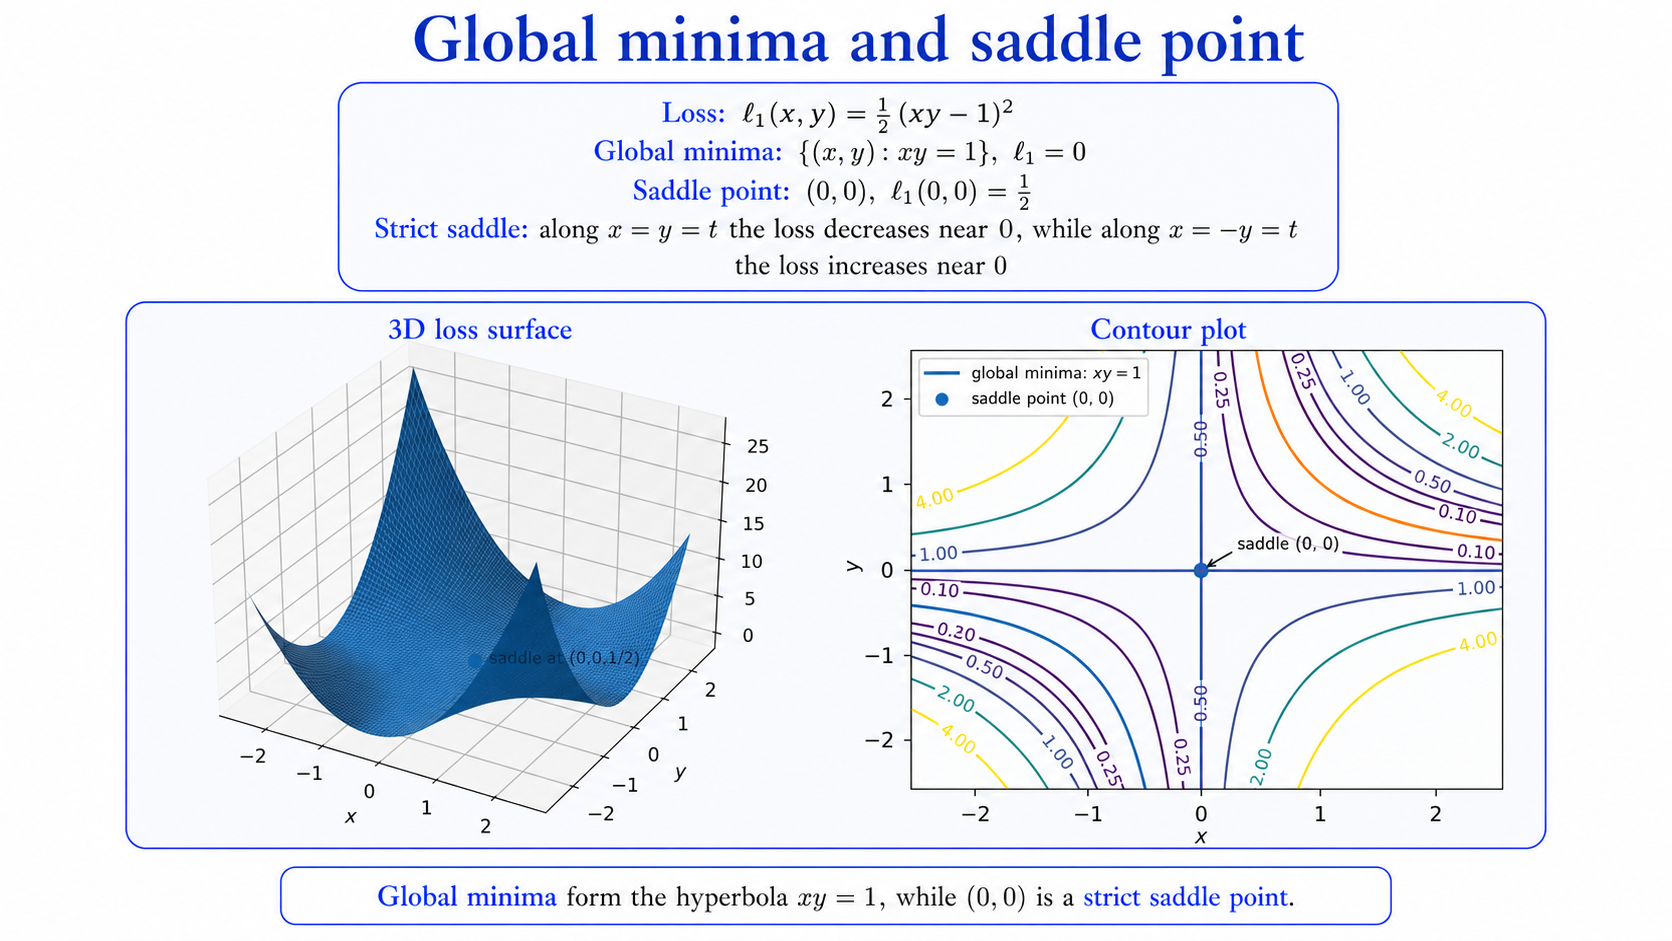
\includegraphics[width=\textwidth,height=\textheight,keepaspectratio]{figures/global_minima_saddle_3d_loss.png}
\end{frame}
\begin{comment}
\begin{frame}
\begin{block}{Example: \(W=\operatorname{diag}(s_1,0)\) is a saddle}
Take a critical point with \(a_1b_1=s_1\) and \(a_2=b_2=0\).

For the perturbation \(a_2=t,\ b_2=t\),
\[
W(t)=\operatorname{diag}(s_1,t^2),
\]
and
\[
\mathcal L(t)-\mathcal L(0)
=
\frac12(t^2-s_2)^2-\frac12s_2^2
=
-s_2t^2+\frac12t^4<0
\]
for small \(t\neq 0\).

For the perturbation \(a_2=t,\ b_2=-t\),
\[
W(t)=\operatorname{diag}(s_1,-t^2),
\]
and
\[
\mathcal L(t)-\mathcal L(0)
=
\frac12(-t^2-s_2)^2-\frac12s_2^2
=
s_2t^2+\frac12t^4>0.
\]
Thus there are both descending and ascending directions, so this critical point is a saddle.
\end{block}
\end{frame}
\end{comment}
\begin{frame}{Deep learning without poor local minima}
Assume that $\Sigma_X$ and $\Sigma_{YX}$ are full rank, and that $\Sigma_{YX}$ has $d_L$ distinct singular values.
\begin{block}{No non-global local minima}
    The loss function of a DLN of depth $L$ is non-convex and non-concave, and every critical point that is not a global minimum is a saddle point.
\end{block}
The training dynamics cannot get stuck in spurious local minima.
\\
Reference: \textit{Kawaguchi, Kenji. "Deep learning without poor local minima." Advances in neural information processing systems 29 (2016)}
\end{frame}
\begin{frame}{Parametrization of critical points}
Teacher SVD: \(M=U\operatorname{diag}(s_1,\ldots,s_{r_m},0_{d_L-r_m})V^{\top}\).
\begin{block}{Saddle points}
    Let $\theta\in\Omega$ be a critical point of rank $r$. Then there exists a subset $S$ of left singular vectors of $M$ and a projector $P_S=U_S U_S^{\top}$ onto their span such that:
    \[
    \mu(\theta) = P_S M = U_S\operatorname{diag}(s_1,\ldots,s_{r},0_{d_L-r})V^{\top}
    \]
\end{block}
The saddle points are given by a subset of singular values and (left) singular vectors of the teacher $M$.
\\
Reference: \textit{Achour, El Mehdi, François Malgouyres, and Sébastien Gerchinovitz. "The loss landscape of deep linear neural networks: a second-order analysis." Journal of Machine Learning Research 25.242 (2024): 1-76.}
\end{frame}
\begin{frame}{Symmetries}
Let $G_{\mathbf{d}}:=\prod_{\ell=0}^{L} GL_{d_\ell}$ act on $\Omega$ via:
\[
(W_1,\dots,W_L)\mapsto (g_1W_1g_0^{-1},\; g_2W_2g_1^{-1},\;\dots,\; g_L W_L g_{L-1}^{-1}),
\]
\begin{block}{Equivariance of the multiplication map}
    Since \(W_Lg_{L-1}^{-1}g_{L-1}W_{L-1}\cdots g_1^{-1}g_1W_1=W_L\cdots W_1\), the multiplication map $\mu$ is $G_{\mathbf{d}}$-equivariant and $G_h$-invariant:
    \[
    \mu(g\cdot \theta)=g_L W g_0^{-1},
    \qquad
    \mu(g_h\cdot \theta) = \mu(\theta).
    \]
A DLN is degenerate: infinitely many DLNs can map to the same student matrix.
\end{block}
It is natural to study solutions up to $G_d$ symmetries. By equivariance of $\mu$, $G_d$ acts on the determinantal variety
\[
\Sigma_d^{r}:=\{\theta\in \Omega\mid\operatorname{rank}(\mu(\theta)) = r\}.
\]
\end{frame}
\begin{comment}
\begin{frame}{Quiver representation theory}
    \begin{block}{Basic notions}
    A quiver $Q$ is a graph $(I,E,s,t)$ with a map $s(e) = V_{i}$ and $t(e)=V_{i+1}$ when edge $e\in E$ connects vertices $i$ and $i+1$ in $I$. Loops and cycles are allowed.
    \\
    A quiver representation assigns a vector space $V_i$ to each $i\in I$ and a linear map $\phi_e$ to each arrow $e\in E$. Note $\text{Rep}_d(Q)$ the space of representations of dimension vector $d=(d_i)_{i\in I}$ 
    \end{block}
Example: The linear quiver $A_n:1\to 2\to ... \to n$ and representation $k\to^{id} k \to^{id} ... \to^{id} k$
\begin{block}{DLN as quiver representations}
The multiplication map of a DLN $\mu$ is a map from $\text{Rep}_d(A_{L+1})\to \operatorname{Mat}_{d_L\times d_0}$ with linear maps given by weight matrices $W_i$ and vector space $\mathbb{R}^{d_i}$. 
\end{block}
In particular $\Sigma_d^r$ is a subvariety of $\text{Rep}_d(A_{L+1})$.
\end{frame}
\end{comment}
\begin{frame}[plain]
\centering
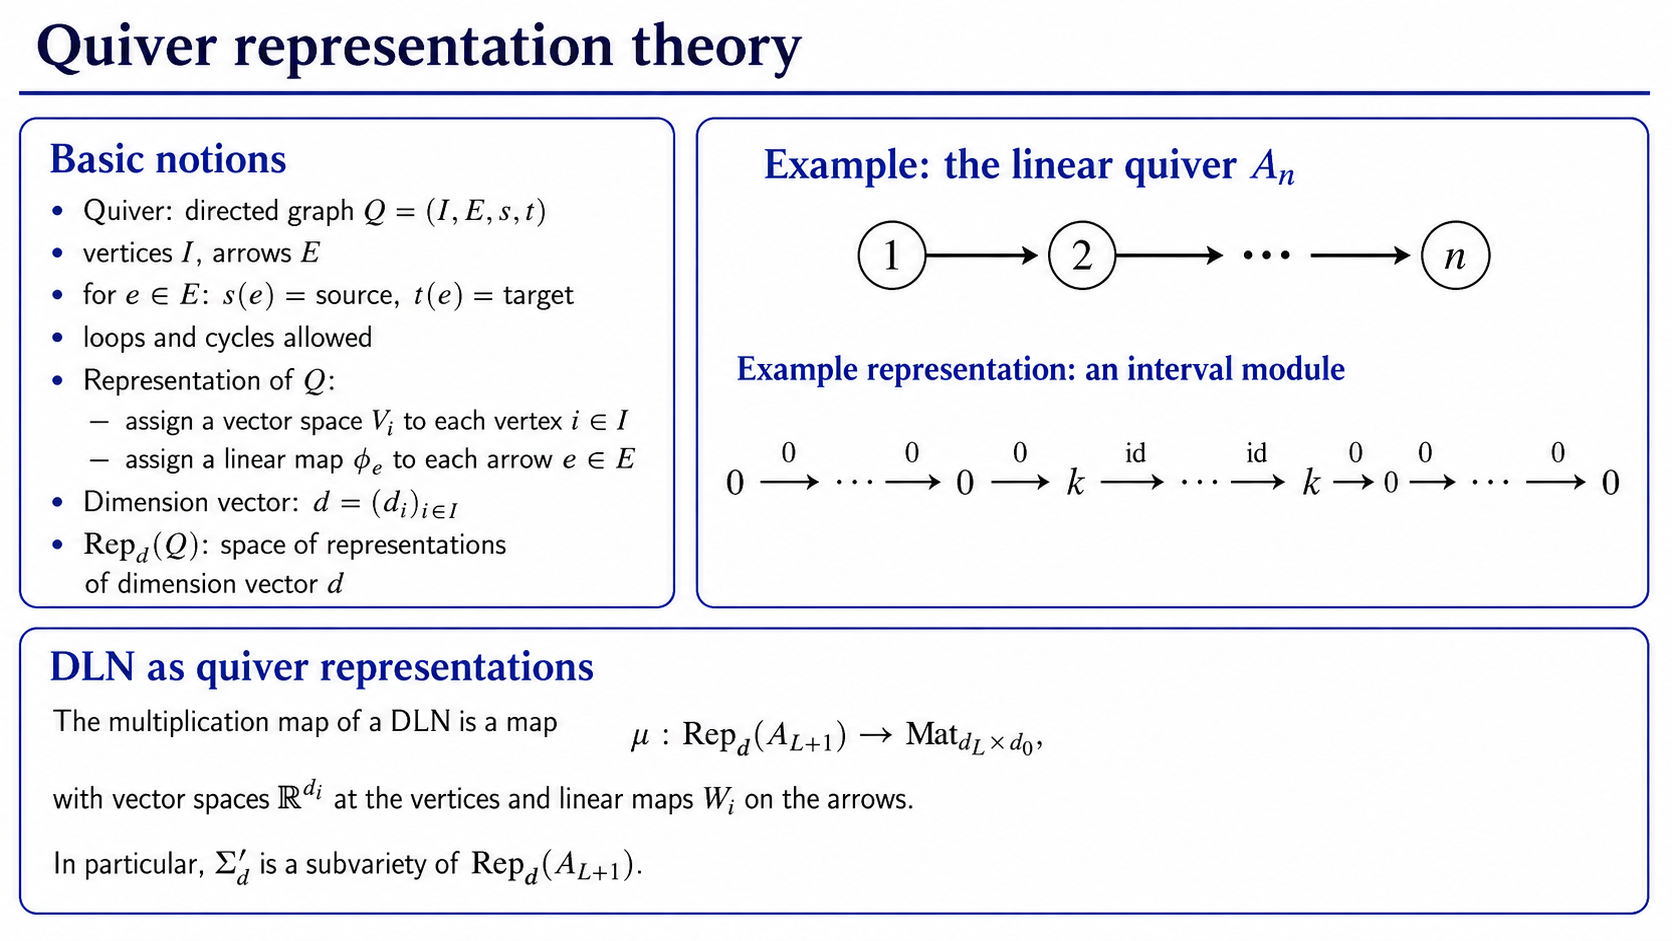
\includegraphics[width=\textwidth,height=\textheight,keepaspectratio]{figures/quiver_representation_theory.png}
\end{frame}
\begin{frame}[plain]
\centering
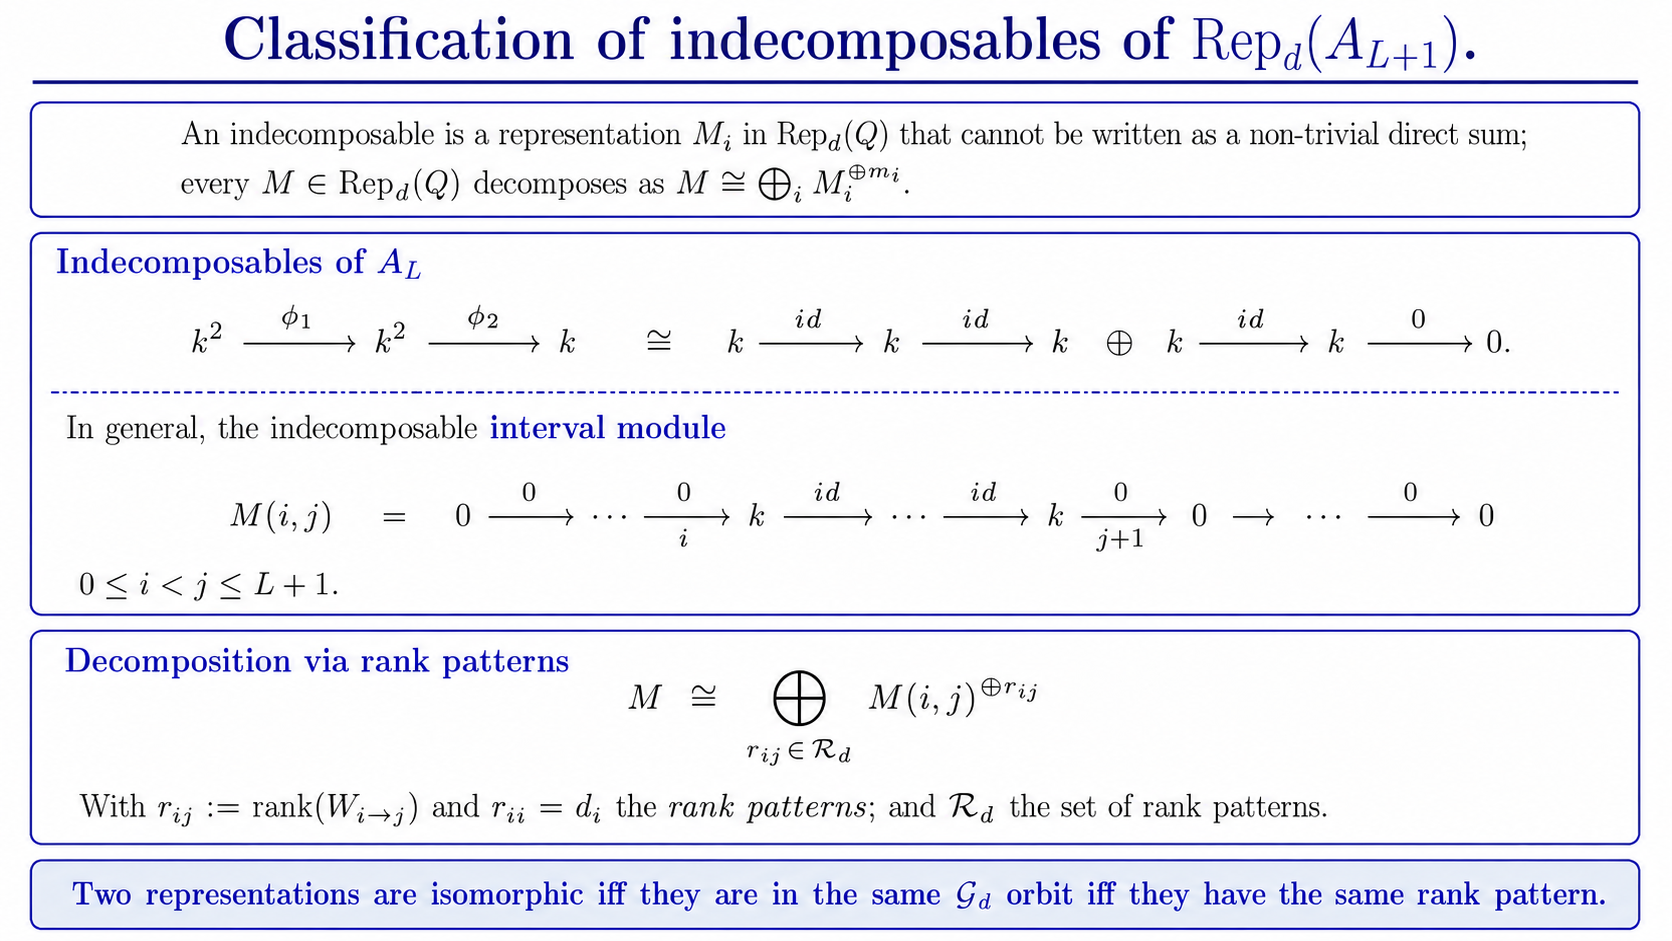
\includegraphics[width=\textwidth,height=\textheight,keepaspectratio]{figures/indecomposables_linear_quiver.png}
\end{frame}
\begin{comment}
\begin{frame}{Classification of indecomposables of ${Rep}_d(A_{L+1})$}
Indecomposable is smallest $M_i \in \text{Rep}_d(Q) $ such that $M \cong \bigoplus M_i^{m_i}$ for $M\in\text{Rep}_d(Q)$ 
\begin{block}{Indecomposables of $A_L$}
Example: $k^2 \to^{\phi_1} k^2 \to^{\phi_2} k \cong k \to^{id} k \to^0 0 \oplus k \to^{id} k \to^0 0$.
\\
More generally all indecomposables are of the form:
$M(i,j) = 0\to^{0} ... \to^{0}_i k \to^{id} ... \to^{id} k \to^{0}_{j+1} 0 \to ... \to^{0} 0 $ for $0\leq i < j \leq L + 1$ 
\\
See: Gabriel Theorem for Dynkin quivers.     
\end{block}
\begin{block}{Decomposition via rank patterns}
Krull-Schmidt and Gabriel theorem $\implies$ for all $M\in \text{Rep}_d(A_{L+1})$ we have a unique decomposition:
\[
M \cong \bigoplus_{r_{ij}\in \mathcal{R}_d} M(i,j)^{\oplus r_{ij}}
\]
With $r_{ij} := \operatorname{rank}(W_{i\to j})$ and $r_{ii}=d_i$ the \textit{rank patterns}; and $\mathcal{R}_d$ the set of rank patterns (with some constraints)
\end{block}
\end{frame}
\end{comment}
\begin{frame}{Stratification of the determinantal variety}
\begin{block}{Orbits are parameterized by rank patterns}
The $G_d$-orbits in $\Sigma_d^r$ are indexed by rank patterns:
\[
\Sigma_d^r = \bigsqcup_{\rho\in \mathcal{R}^r_d} \mathcal{O}_{\rho}
\]
Two representations are in the same $G_d$-orbit if and only if they are isomorphic, equivalently if and only if they have the same decomposition into indecomposables.
\\
Thus rank patterns stratify $\Sigma_d^r$. Since $\Sigma_d^{r_m} = G_{\text{out}}\cdot\mu^{-1}(M)$, this gives a combinatorial description of the global minima.
\end{block}
Rank patterns are natural observable geometric invariants for DLNs.
\end{frame}
\begin{frame}{Link with SLT}
\begin{block}{Codimension of the global minima}
For a teacher matrix $M$ of rank $r_m$, we have:
    \[
    \begin{aligned}
    \operatorname{codim}_{\operatorname{Rep}_d}(\mu^{-1}(M))
    &=
    \operatorname{codim}_{\operatorname{Rep}_d}(\Sigma_d^{r_m})
    + r_m(d_0 - d_L - r_m) \\
    &= 2\operatorname{RLCT}(\mathcal{L}^{-1})(0).
    \end{aligned}
    \]
In general, we only have:
\[
\operatorname{RLCT}(\mathcal{L}^{-1})(0)  \leq \frac{1}{2}\operatorname{codim}_{\operatorname{Rep}_d}(\mathcal{L}^{-1}(0)).
\]
\end{block}
Ref: \textit{Lehalleur, Simon Pepin, and Richárd Rimányi. "Geometry of fibers of the multiplication map of deep linear neural networks." arXiv preprint arXiv:2411.19920 (2024).}
\end{frame}
\begin{frame}{Discussion}
\begin{block}{Takeaways}
Under full-rank and nondegenerate-data assumptions:
    \begin{itemize}
        \item Critical points of DLNs are either saddles or global minima
        \item Gauge symmetries mean there is a whole algebraic variety of degenerate minima
        \item Quiver representation theory gives a combinatorial description of the global minima
        \item The codimension of the global minima is twice the RLCT
    \end{itemize}
\end{block}
\end{frame}
\begin{frame}{References}
\begin{itemize}
    \item Kenji Kawaguchi. Deep learning without poor local minima \textit{Advances in neural
information processing systems}, 29, 2016.
    \item El Mehdi Achour, François Malgouyres, and Sébastien Gerchinovitz. The loss
landscape of deep linear neural networks: a second-order analysis. \textit{Journal of
Machine Learning Research}, 25(242):1–76, 2024.
    \item Anna Choromanska, Mikael Henaff, Michael Mathieu, Gérard Ben Arous, and
Yann LeCun. The loss surfaces of multilayer networks. In \textit{Artificial intelligence
and statistics}, pages 192–204. PMLR, 2015.
    \item Lehalleur, Simon Pepin and Rim{\'a}nyi, Rich{\'a}rd. Geometry of fibers of the multiplication map of deep linear neural networks, arXiv preprint arXiv:2411.19920, 2024.
    \item Chen, Po and Jiang, Rujun and Wang, Peng. A Complete Loss Landscape Analysis of Regularized Deep Matrix Factorization, arXiv preprint arXiv:2506.20344, 2025.
\end{itemize}
\end{frame}
\begin{frame}
    \begin{center}
        Dynamics 
    \end{center}
\end{frame}
\begin{frame}{Gradient Flow}
\begin{block}{Two-layer DLN}
\begin{align*}
    W &:= W_2W_1, &
    R(W) &:= \Sigma_{YX}-W_2W_1 .
\end{align*}

For the population loss
\[
    \mathcal{L}(W_1,W_2)=\frac{1}{2}\lVert\Sigma_{YX}-W_2W_1\rVert_F^2,
\]
gradient flow is
\begin{align*}
    \dot{W}_1 &= W_2^{\top}R(W),\\
    \dot{W}_2 &= R(W)W_1^{\top}.
\end{align*}
\end{block}
\end{frame}
\begin{frame}[plain]
\centering
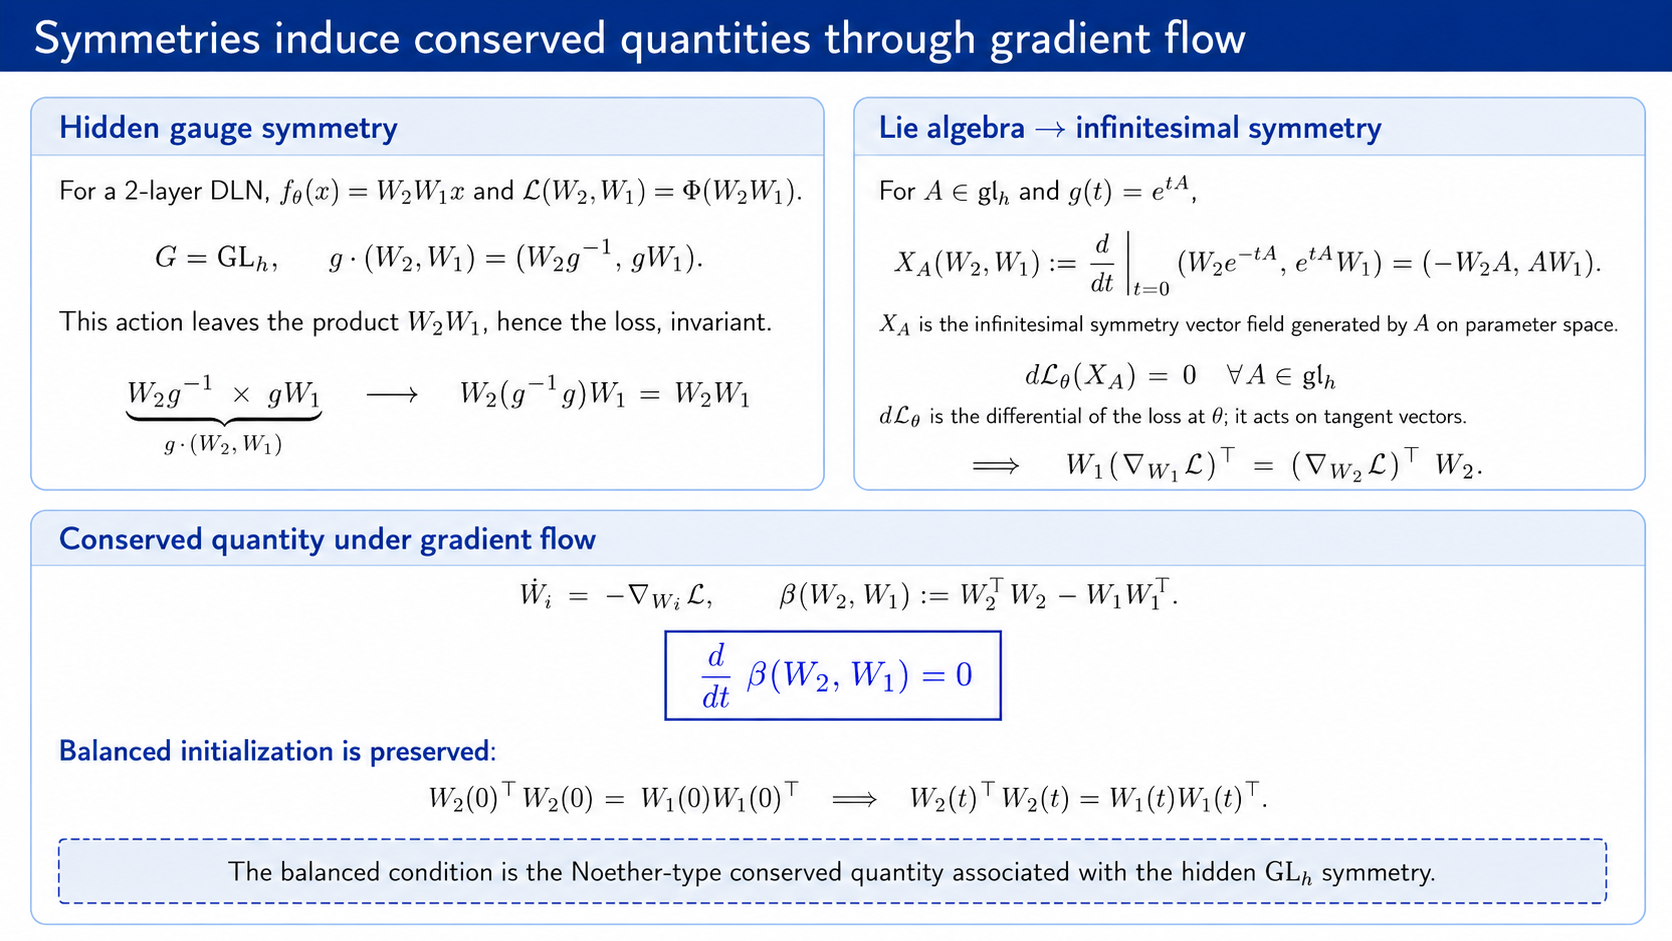
\includegraphics[width=\paperwidth,height=\paperheight,keepaspectratio]{figures/conserved_quantities.png}
\end{frame}
\begin{frame}[plain]
\centering
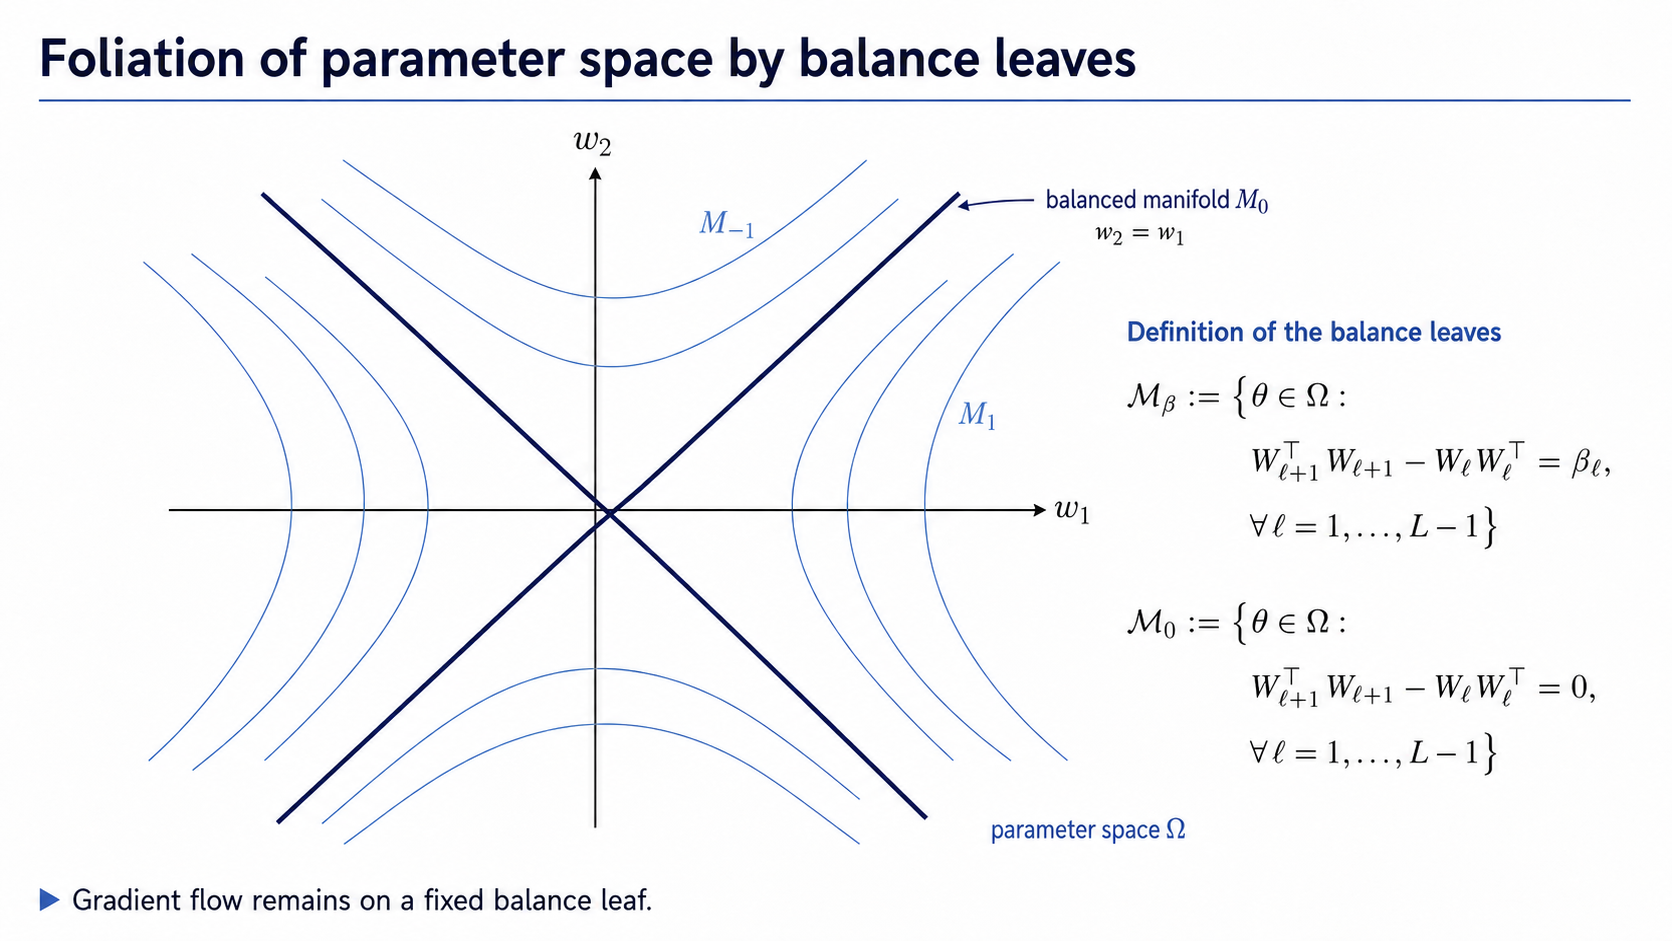
\includegraphics[width=\textwidth,height=\textheight,keepaspectratio]{figures/foliation_paramaters_balanced.png}
\end{frame}
\begin{frame}[plain]
\centering
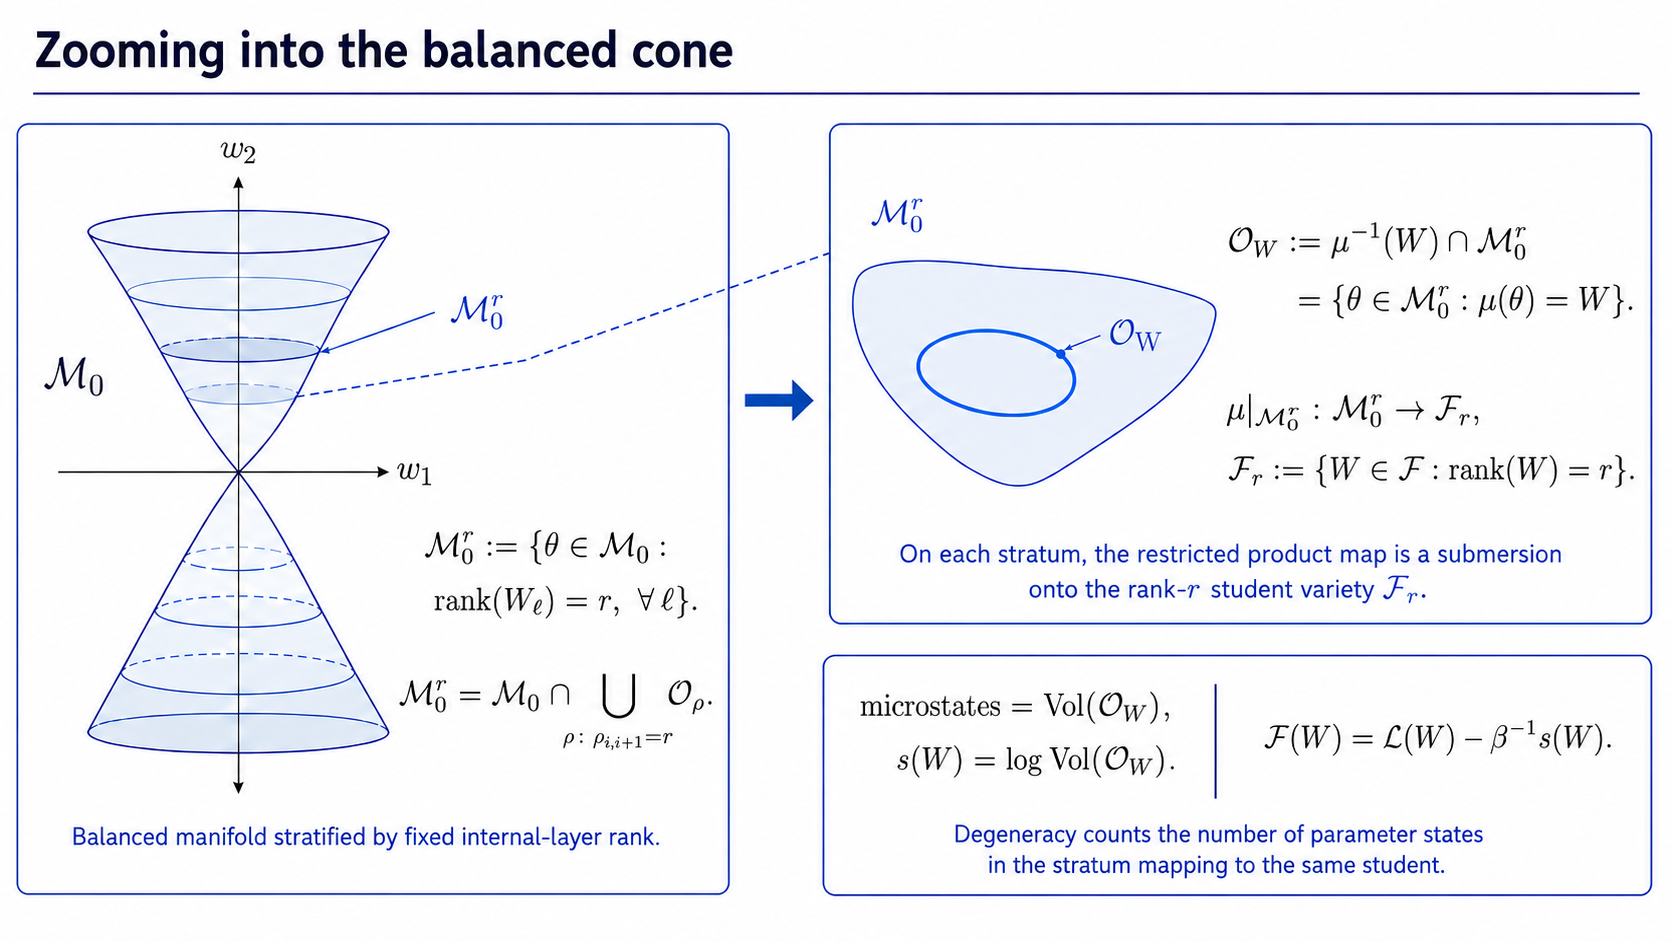
\includegraphics[width=\textwidth,height=\textheight,keepaspectratio]{figures/balanced_cone_micro_states.png}
\end{frame}
\begin{comment}
\begin{frame}{Foliation of the balance manifold}
    The conserved balanced quantities
\[
B_\ell(\theta)
=
W_{\ell+1}^{\top}W_{\ell+1}
-
W_\ell W_\ell^{\top}
\]
define level sets
\[
\mathcal M_G = B^{-1}(\beta).
\]
Thus parameter space decomposes as
\[
\Omega=\bigsqcup_G \mathcal M_G.
\]
Since \(\frac{d}{dt}B_\ell(\theta(t))=0\) along gradient flow, each flow is contained
\(\mathcal M_G\) is invariant through the flow.
\end{frame}
\begin{frame}
    \begin{block}{Rank strata inside the balanced leaf}
On the balanced leaf \(\mathcal M_0\),
\[
    W_{\ell+1}^{\top}W_{\ell+1}
    =
    W_\ell W_\ell^{\top}.
\]
Hence consecutive layers have the same singular values, and therefore the same rank.
Thus
\[
    \mathcal M_0
    =
    \bigsqcup_r \mathcal M_r,
    \qquad
    \mathcal M_r
    :=
    \{\theta\in\mathcal M_0:\operatorname{rank}(W_\ell)=r\ \forall \ell\}=\mathcal M_0 \cap \mathcal{O}_{\rho_{i,i+1} = r}
\]
Moreover,
\[
    \mu(\mathcal M_r)
    =
    \mathcal F_r
    :=
    \{W\in\mathcal F:\operatorname{rank}(W)=r\}.
\]
Balanced rank-\(r\) parameter leaf projects to the rank-\(r\) stratum of
function space.
\end{block}
\end{frame}
\end{comment}
\begin{frame}{The manifold of gradient flow}
Gradient flow is constrained on the following hyperbolic manifold:
\begin{equation*}
    \mathcal{M}_{\beta} := \{\theta\in\Omega\mid W_{\ell+1}^{\top}W_{\ell+1} - W_{\ell}W_{\ell}^{\top} = \beta_\ell\}
\end{equation*}
\begin{block}{Gradient flow on the balanced variety}
On the balanced variety $\mathcal{M}_0$, the self-consistent gradient flow equation in function space is
\begin{equation*}
    \dot{W}
    =
    \sum_{k=1}^{L}
    (WW^{\top})^{\frac{L-k}{L}}
    R(W)
    (W^{\top}W)^{\frac{k-1}{L}},
    \qquad
    R(W):=\Sigma_{YX}-W.
\end{equation*}
For depth $2$:
\[
    \mathcal{M}_0
    =
    \{(W_1,W_2)\mid W_2^{\top}W_2=W_1W_1^{\top}\}.
\]
\begin{equation*}
    \dot{W}
    =
    (WW^{\top})^{\frac{1}{2}}R(W)
    +
    R(W)(W^{\top}W)^{\frac{1}{2}}.
\end{equation*}
\end{block}
\end{frame}
\begin{frame}[plain]
\centering
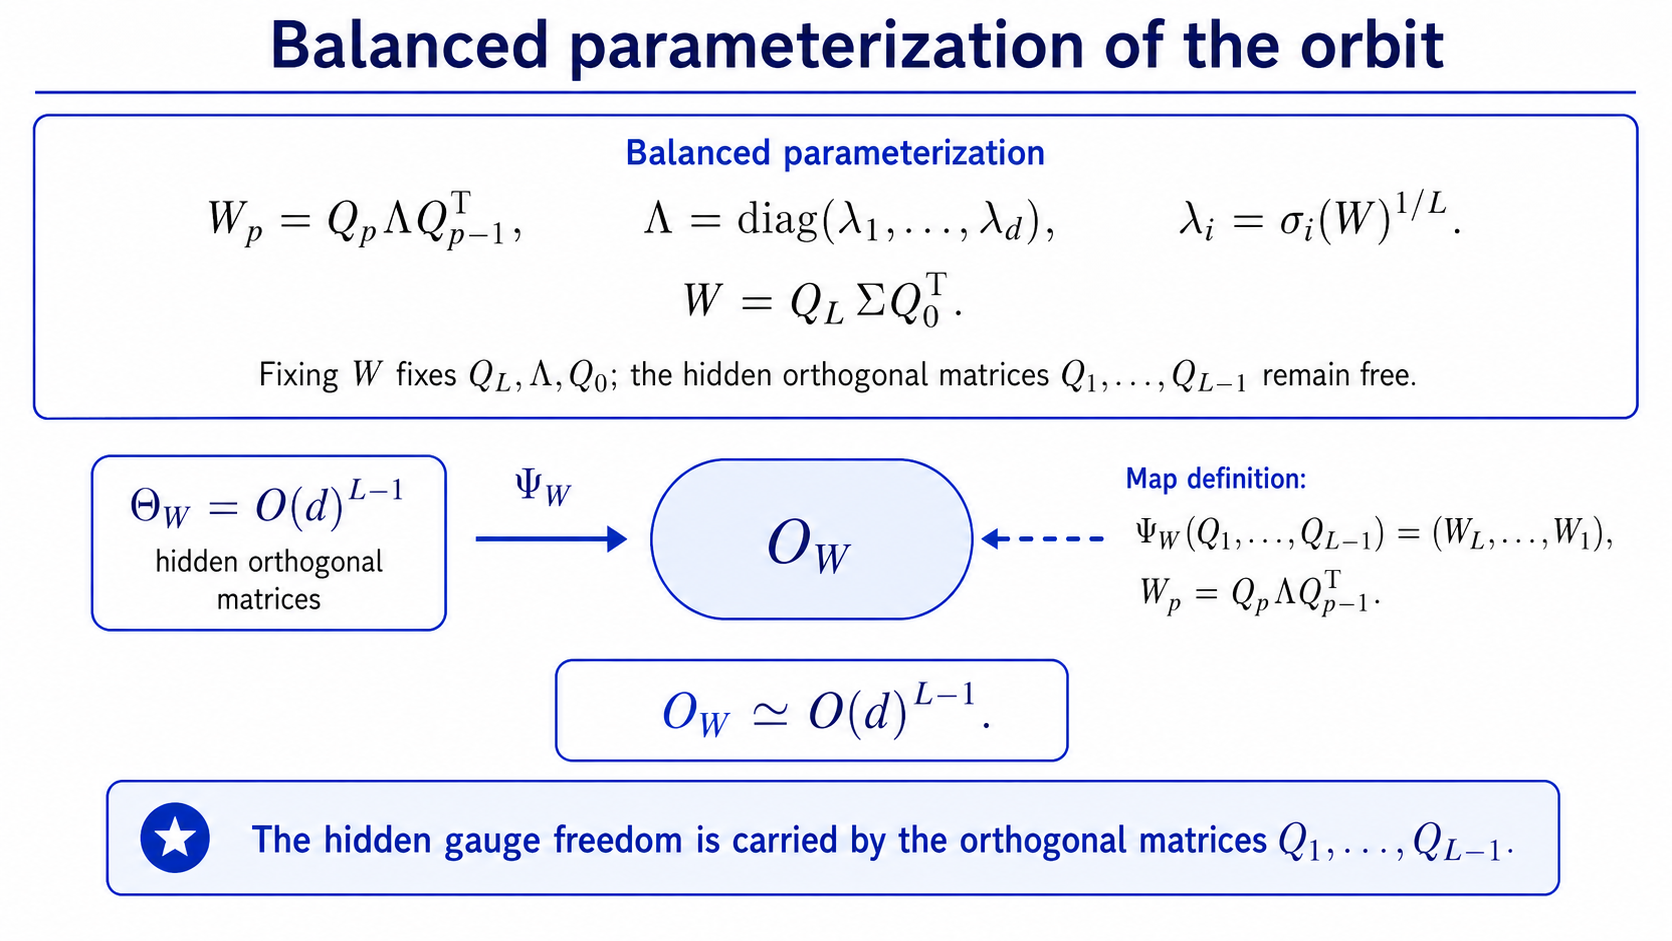
\includegraphics[width=\textwidth,height=\textheight,keepaspectratio]{figures/balanced_parametrization.png}
\end{frame}
\begin{comment}
\begin{frame}[plain]
\centering
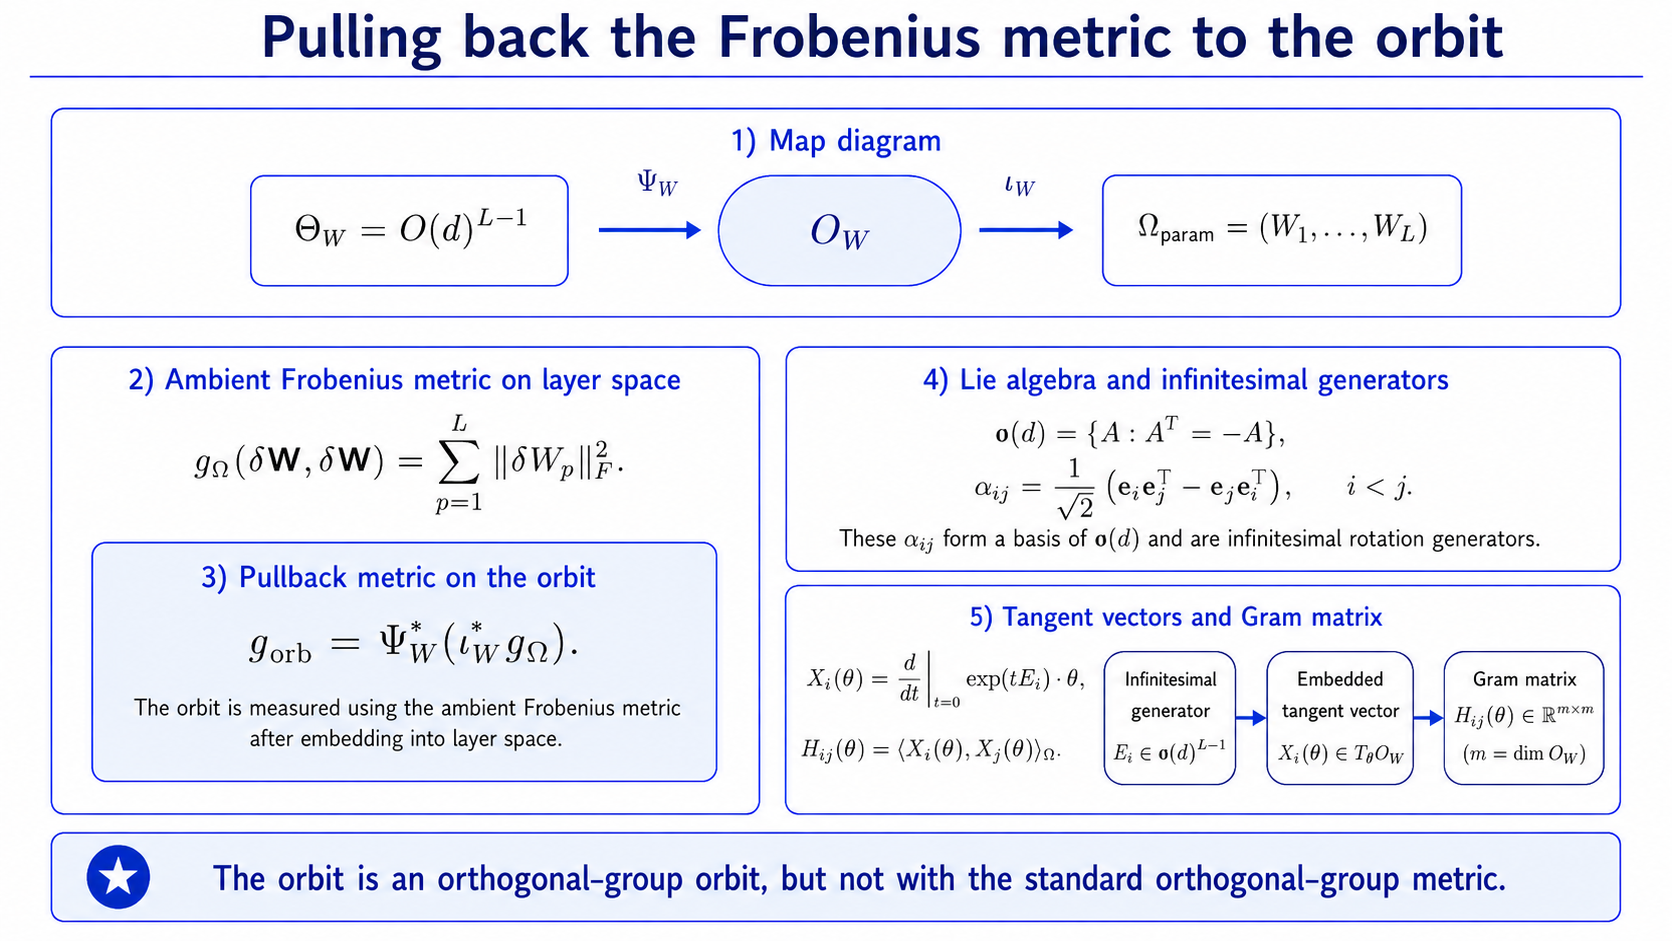
\includegraphics[width=\textwidth,height=\textheight,keepaspectratio]{figures/frobenius_pull_back.png}
\end{frame}
\end{comment}
\begin{frame}[plain]
\centering
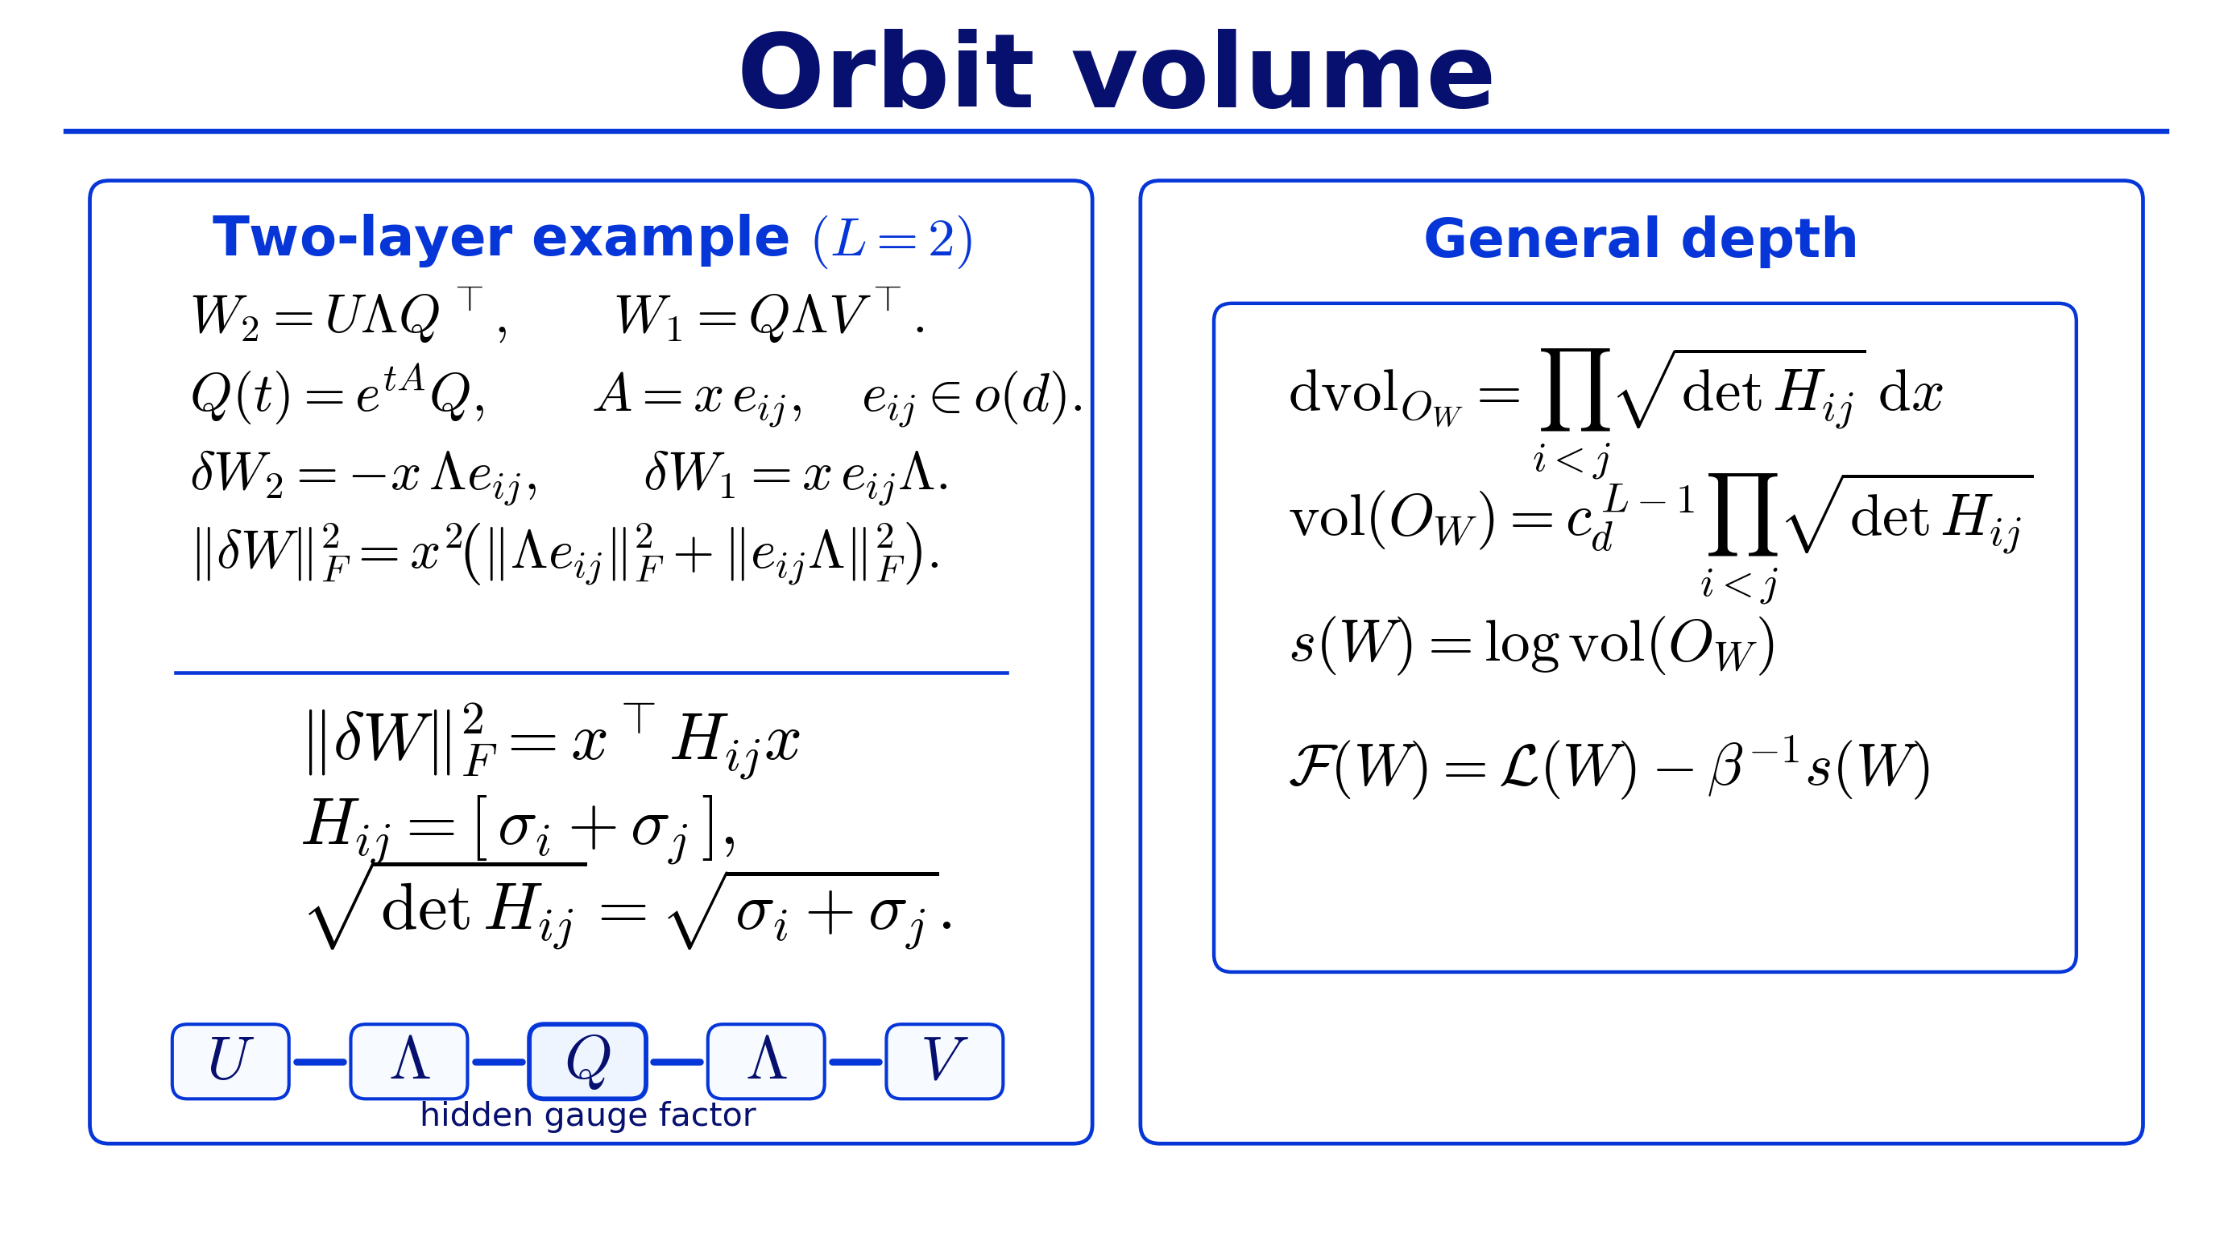
\includegraphics[width=\textwidth,height=\textheight,keepaspectratio]{figures/orbit_volume.png}
\end{frame}
\begin{comment}
\begin{frame}{Riemannian flow}
    \begin{block}{Why the projected flow is Riemannian}
On a balanced rank stratum \(\mathcal M_r\), the product map
\[
    \mu:\mathcal M_r\to\mathcal F_r
\]
is a Riemannian submersion when \(\mathcal F_r\) is equipped with the induced metric
\[
    \|Z\|_{g_L,W}^2
    =
    \min_{D\mu_\theta[\dot\theta]=Z}
    \sum_{\ell=1}^L \|\dot W_\ell\|_F^2 .
\]
Since \(\mathcal L\circ\mu\) is constant along the fibers of \(\mu\), its Euclidean gradient is
horizontal. Therefore
\[
    D\mu_\theta[\nabla_\theta(\mathcal L\circ\mu)]
    =
    \operatorname{grad}_{g_L}\mathcal L(W),
\]
and the parameter gradient flow projects to
\[
    \dot W=-\operatorname{grad}_{g_L}E(W).
\]
\end{block}
\end{frame}
\begin{frame}
    \begin{block}{From energy to free energy}
The product map has fibers
\[
    \mathcal O_W:=\mu^{-1}(W)\cap\mathcal M_r ,
\]
i.e. many parameter microstates represent the same function \(W\).
Their volume defines a Boltzmann entropy
\[
    S(W):=\log\operatorname{vol}(\mathcal O_W).
\]
With microscopic fluctuations along the fibers, the effective macroscopic objective is
\[
    F_\beta(W)=E(W)-\frac1\beta S(W).
\]
Thus the Riemannian energy flow is replaced by free-energy flow:
\[
    \dot W=-\operatorname{grad}_{g_L}F_\beta(W)
    =
    -\operatorname{grad}_{g_L}E(W)
    +\frac1\beta\operatorname{grad}_{g_L}S(W).
\]
\end{block}
\end{frame}
\end{comment}
\begin{comment}
\begin{frame}{Spectral entropy on the balanced manifold}

Balanced layers have the same singular values
\[
\lambda_1,\dots,\lambda_d,
\qquad
\sigma_i=\lambda_i^L.
\]
\begin{block}{Entropy}
Boltzmann entropy of orbit:
\[
S(W):=\log \operatorname{vol}(\mathcal O_W).
\]
Menon formula:
\[
S(W)
=
(L-1)\log c_d
+
\frac12\sum_{i<j}
\log\!\left(
\frac{\lambda_i^{2L}-\lambda_j^{2L}}
     {\lambda_i^2-\lambda_j^2}
\right).
\]
\end{block}

\end{frame}
\end{comment}
\begin{frame}{References}
    \begin{itemize}
        \item Menon, Govind. The geometry of the deep linear network. Symposium on Probability and Stochastic Processes. Cham: Springer Nature Switzerland, 2023.
        \item Sibylle Marcotte, R\'emi Gribonval, and Gabriel Peyr\'e. Abide by the law and
follow the flow: Conservation laws for gradient flows. \textit{Advances in neural
information processing systems}, 36:63210–63221, 2023.
    \item Sanjeev Arora, Nadav Cohen, Noah Golowich, and Wei Hu. \textit{A convergence
analysis of gradient descent for deep linear neural networks}. arXiv preprint
arXiv:1810.02281, 2018
    \item Arthur Jacot, Franck Gabriel, and Cl\'ement Hongler. Neural tangent kernel: Con-
    vergence and generalization in neural networks. \textit{Advances in neural information
    processing systems}, 31, 2018.
    \item Jeremy M Cohen, Alex Damian, Ameet Talwalkar, J Zico Kolter, and Jason D
    Lee. Understanding optimization in deep learning with central flows. arXiv
    preprint arXiv:2410.24206, 2024
    \end{itemize}
\end{frame}
%----------Rich Regime for DLNs-----------
\begin{frame}{Saddle-to-saddle regime in DLNs}
Assume whitened inputs $\Sigma_X = I$ and $\Sigma_{YX} = U S V^{\top}$. Define the layerwise modes of a 2-layer DLN by
\begin{equation*}
    w_1^{\alpha} := W_1 v^{\alpha} \in \mathbb{R}^{d_1}, 
    \qquad
    w_2^{\alpha} := W_2^{\top} u^{\alpha} \in \mathbb{R}^{d_1},
\end{equation*}
The DLN mode matrix is
\begin{equation*}
    w_{\alpha\beta}=u^{\alpha\top} W_2 W_1 v^{\beta} = (w_2^{\alpha})^{\top} w_1^{\beta}.
\end{equation*}
Assuming gradient flow on the balanced manifold and using the self-consistent gradient-flow equation:
\begin{equation*}
    \dot{w}_{\alpha\alpha} = 2\left(s_{\alpha} - w_{\alpha\alpha}\right)w_{\alpha\alpha}
    - 2\sum_{\beta\neq\alpha} \left(w_{\alpha\beta}\right)^2 .
\end{equation*}
\end{frame}
\begin{comment}
\begin{frame}{Rich regime in DLNs}
We neglect the cross-mode terms $w_{\alpha\beta}$ (weights are aligned).
\begin{block}{Logistic feature learning}
    For balanced and aligned weights, GF reduces to a system of 1D logistic ODEs:
\begin{equation*}
    \dot{w}_{\alpha} = 2\left(s_{\alpha} - w_{\alpha}\right)w_{\alpha}.
\end{equation*}
Solving this ODE for $w(t):=w_{\alpha}$ gives:
\begin{equation*}
    w(t)=\frac{s}{1+\left(\frac{s}{w_0}-1\right)e^{-2s t}}.
\end{equation*}
\end{block}
\end{frame}
\end{comment}
\begin{comment}
\begin{frame}{Time scale of learning in the rich regime}
 The elapsed time to go from $w_0$ to $w_f$ is
\[
t=\frac{1}{2s}\,\ln\!\left(\frac{w_f\,(s-w_0)}{w_0\,(s-w_f)}\right), \qquad s\neq 0.
\]
For depth $L$:
\[
t=\frac{1}{L} \left[ \frac{1}{s^{2}} \ln\!\left(\frac{w_f\,(s - w_0)}{w_0\,(s - w_f)}\right)
+ \frac{1}{s\,w_0} - \frac{1}{s\,w_f} \right].
\]
\begin{block}{Rich regime}
\begin{itemize}
    \item Stagewise learning ordered by the magnitude of singular values
    \item Saddle to saddle dynamics: GF goes from low to high rank saddles
    \item Simplicity bias of gradient flow and low-hanging fruit prior
\end{itemize}
\end{block}
\end{frame}
\end{comment}
\begin{frame}[plain]
\centering
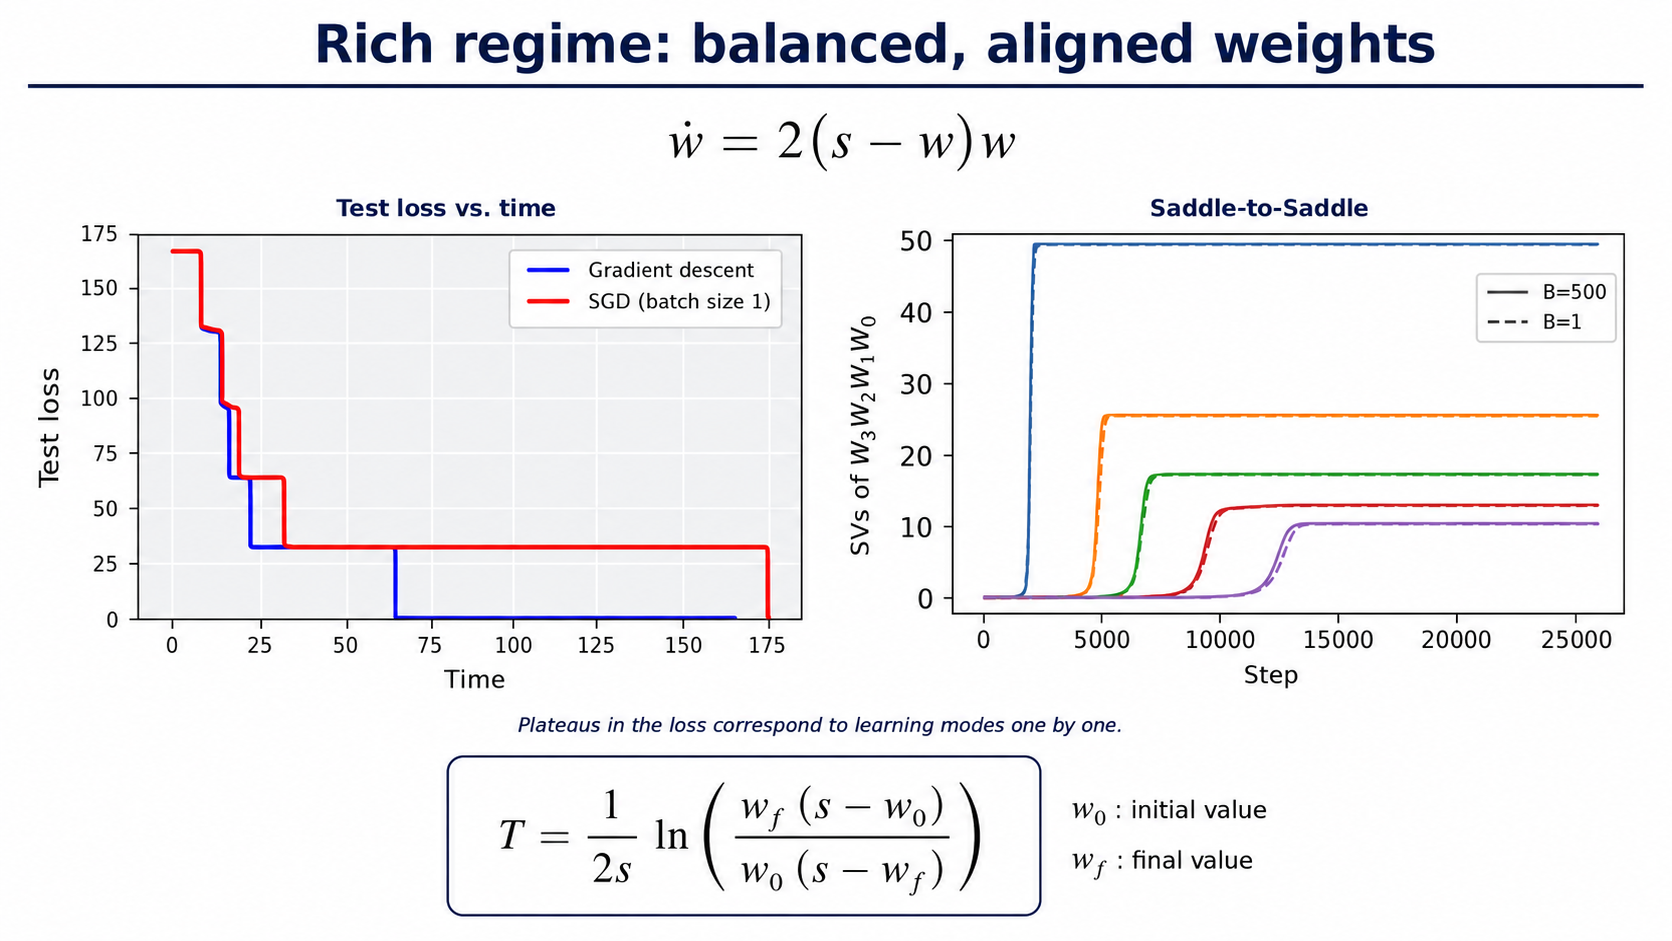
\includegraphics[width=\textwidth,height=\textheight,keepaspectratio]{figures/rich_regime.png}
\end{frame}
\begin{frame}[plain]
\centering
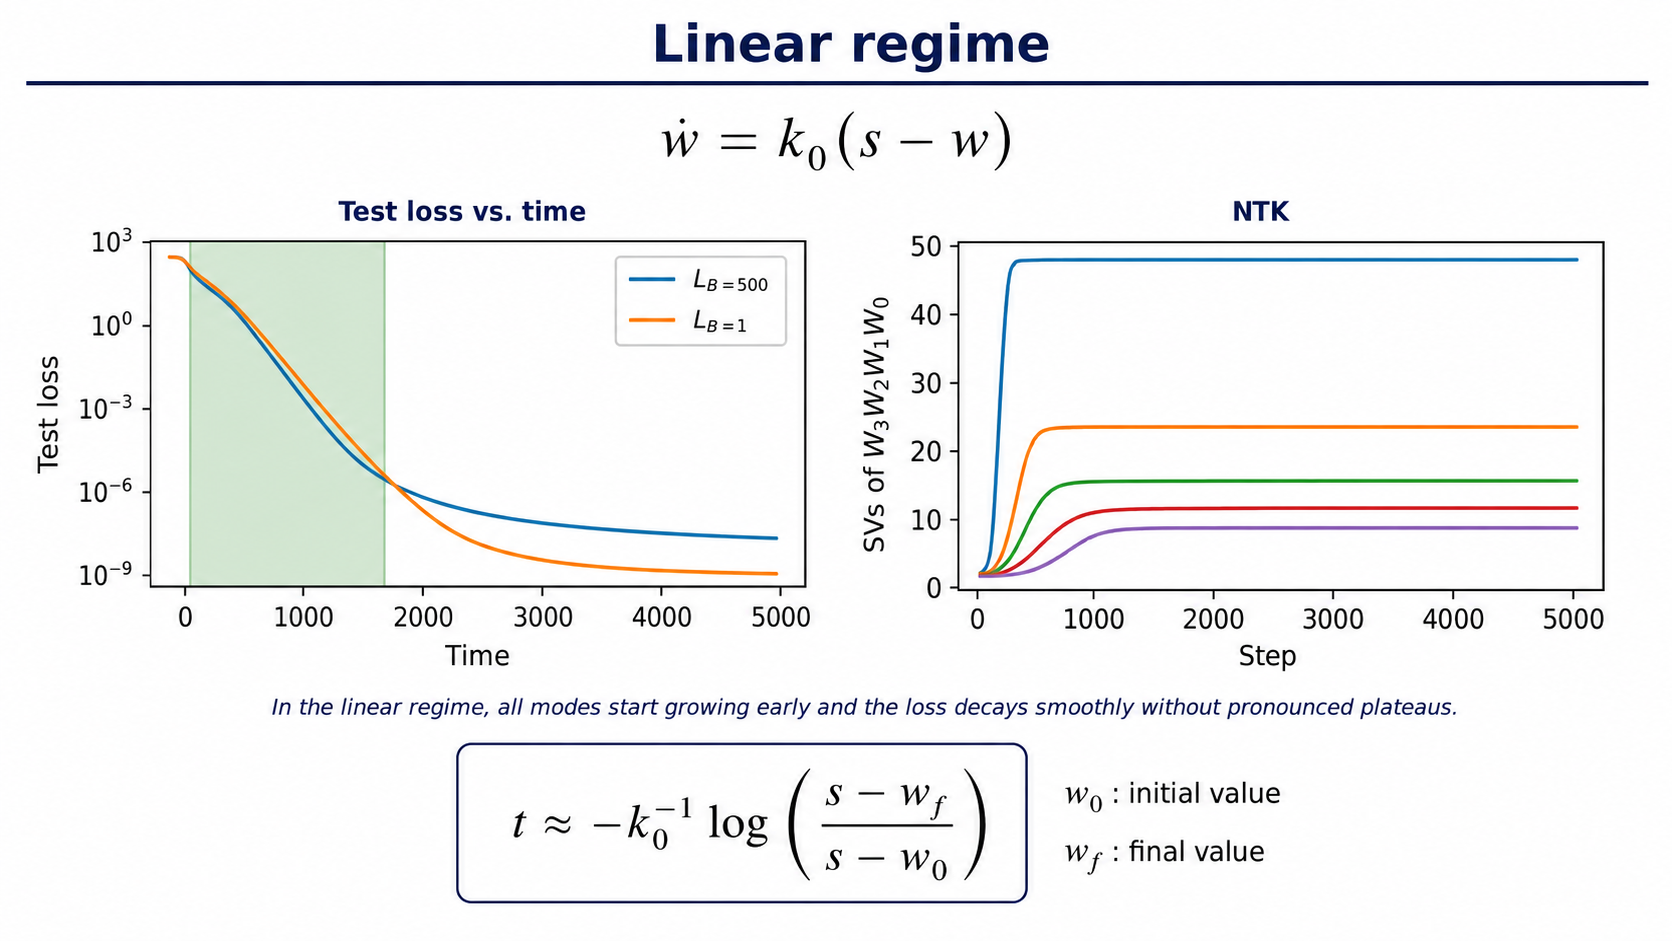
\includegraphics[width=\textwidth,height=\textheight,keepaspectratio]{figures/linear_regime.png}
\end{frame}
\begin{comment}
%----------Lazy Regime for DLNs-----------
\begin{frame}{Linear regime in DLNs}
\begin{block}{Proposition}
For a DLN of depth $L$ in the large width limit, or with a large initialization, we have:
    \begin{align*}
    \dot{W} & \approx K_0[M - W]
\end{align*}
Leading to the following solution:
\begin{equation*}
    W(t) = M - \exp(-K_0 t)[M - W(0)]
\end{equation*}
\end{block}
The time scale of learning is mostly fixed by the NTK at initialization:
\begin{equation*}
    t \approx -k_0^{-1}\log\left(\frac{s - w_f}{s - w_0}\right)
\end{equation*}
No stagewise learning, the structure of the data barely influences the training dynamics, behaves like a linear network.
\end{frame}
\end{comment}
\begin{frame}{References}
    \begin{itemize}
        \item Saxe, Andrew M., James L. McClelland, and Surya Ganguli. A mathematical theory of semantic development in deep neural networks. \textit{Proceedings of the National Academy of Sciences} 116.23 (2019): 11537-11546.
        \item Jacot, Arthur, et al. Saddle-to-saddle dynamics in deep linear networks: Small initialization training, symmetry, and sparsity. \textit{arXiv preprint} arXiv:2106.15933 (2021).
        \item Dominé, Clémentine CJ, et al. From lazy to rich: Exact learning dynamics in deep linear networks. \textit{arXiv preprint} arXiv:2409.14623 (2024)
        \item Zhang, Yedi, Andrew Saxe, and Peter E. Latham. Saddle-to-Saddle Dynamics Explains A Simplicity Bias Across Neural Network Architectures. \textit{arXiv preprint} arXiv:2512.20607 (2025).
        \item Zhenfeng Tu, Santiago Tomas Aranguri Diaz, and Arthur Jacot. Mixed dynamics
in linear networks: Unifying the lazy and active regimes. \textit{Advances in Neural
Information Processing Systems}, 37:106059–106104, 2024.
    \end{itemize}
\end{frame}
\begin{frame}{Discussion}
    \begin{itemize}
    \item DLNs are mathematically tractable and informative about deep learning
    \item Useful for understanding implicit biases from depth, scale, overparameterization, hyperparameters, and optimizers
    \item Symmetries and conserved quantities are central
    \item Different regimes of training dynamics: rich vs.\ lazy
    \item However, they are limited: they cannot learn nonlinear compositional structure
\end{itemize}
\end{frame}
\begin{frame}{Research directions}
    \begin{itemize}
        \item Combinatorial description of all critical points (work in progress)
        \item Generalize the volume formula to the rank-deficient case
        \item Volume formula for the transient saddle-to-saddle regime
        \item Loss landscapes of nonlinear networks (ReLU)
        \item Geometric invariants for nonlinear networks
        \item Toy models of hierarchical learning (nonlinearities)
    \end{itemize}
\end{frame}
\begin{frame}
    Topics we did not discuss:
    \begin{itemize}
        \item Data distribution
        \item Nonlinearities (gated DLNs)
        \item Stochasticity
        \item Discrete learning rate
        \item Scale and statistical field theory
    \end{itemize}
\end{frame}
\begin{frame}[plain]
\centering
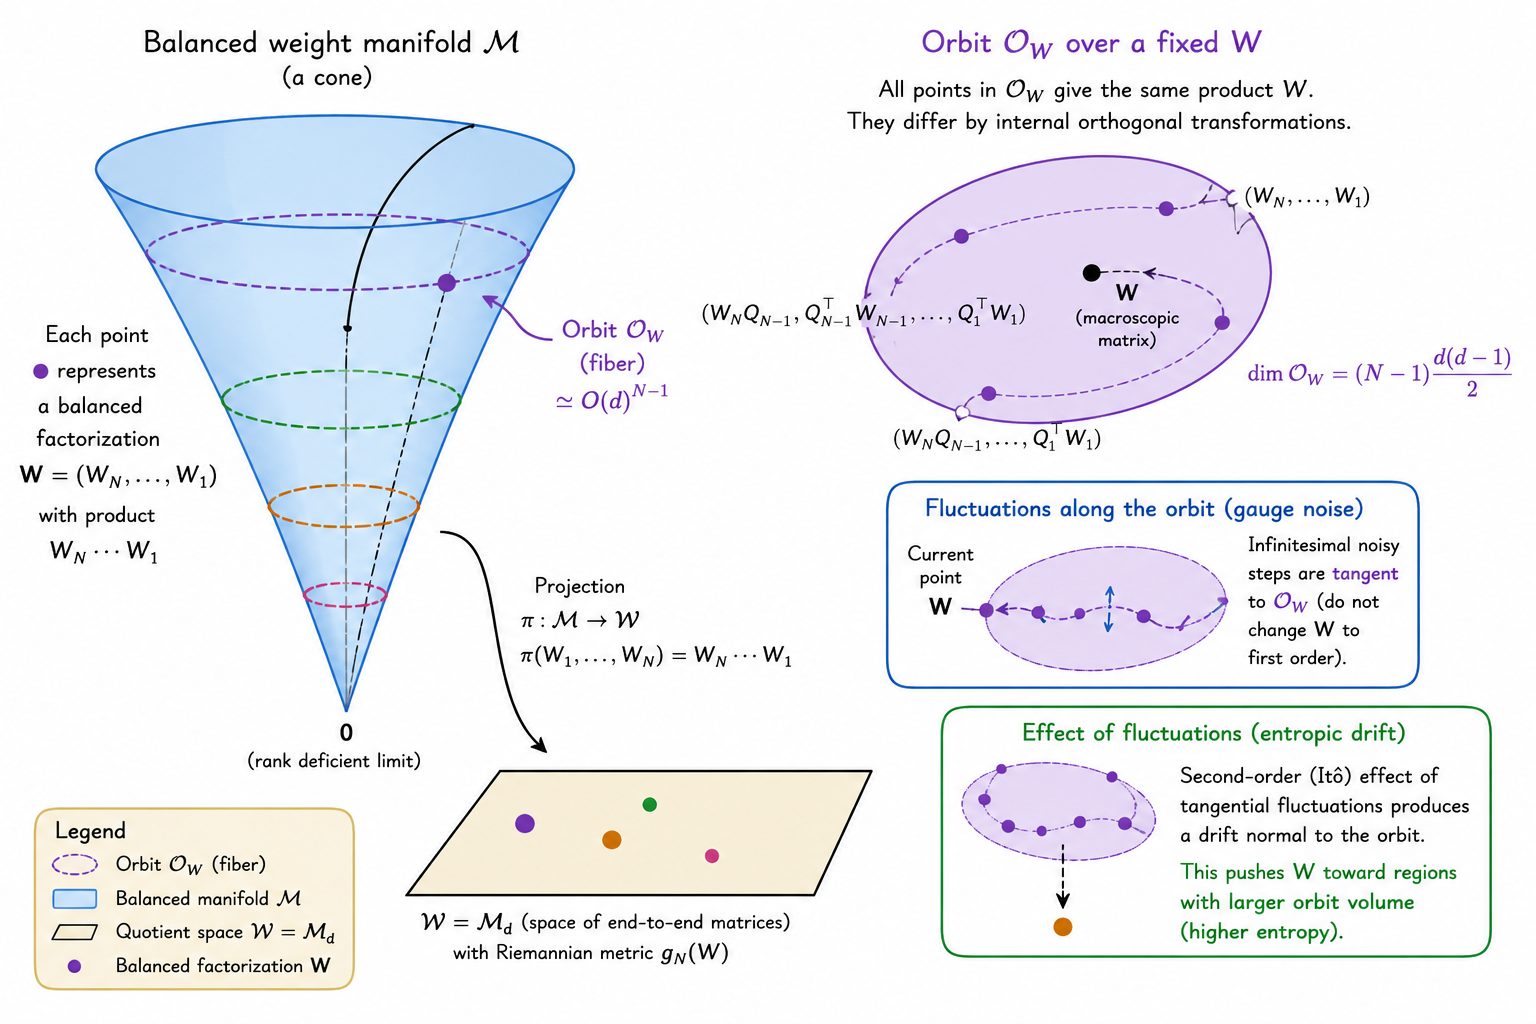
\includegraphics[width=\textwidth,height=\textheight,keepaspectratio]{figures/summary_menon.png}
\end{frame}
\end{document}
